% Options for packages loaded elsewhere
\PassOptionsToPackage{unicode}{hyperref}
\PassOptionsToPackage{hyphens}{url}
%
\documentclass[
  10pt,
]{article}
\usepackage{amsmath,amssymb}
\usepackage{iftex}
\ifPDFTeX
  \usepackage[T1]{fontenc}
  \usepackage[utf8]{inputenc}
  \usepackage{textcomp} % provide euro and other symbols
\else % if luatex or xetex
  \usepackage{unicode-math} % this also loads fontspec
  \defaultfontfeatures{Scale=MatchLowercase}
  \defaultfontfeatures[\rmfamily]{Ligatures=TeX,Scale=1}
\fi
\usepackage{lmodern}
\ifPDFTeX\else
  % xetex/luatex font selection
\fi
% Use upquote if available, for straight quotes in verbatim environments
\IfFileExists{upquote.sty}{\usepackage{upquote}}{}
\IfFileExists{microtype.sty}{% use microtype if available
  \usepackage[]{microtype}
  \UseMicrotypeSet[protrusion]{basicmath} % disable protrusion for tt fonts
}{}
\makeatletter
\@ifundefined{KOMAClassName}{% if non-KOMA class
  \IfFileExists{parskip.sty}{%
    \usepackage{parskip}
  }{% else
    \setlength{\parindent}{0pt}
    \setlength{\parskip}{6pt plus 2pt minus 1pt}}
}{% if KOMA class
  \KOMAoptions{parskip=half}}
\makeatother
\usepackage{xcolor}
\usepackage[margin=22mm]{geometry}
\usepackage{color}
\usepackage{fancyvrb}
\newcommand{\VerbBar}{|}
\newcommand{\VERB}{\Verb[commandchars=\\\{\}]}
\DefineVerbatimEnvironment{Highlighting}{Verbatim}{commandchars=\\\{\}}
% Add ',fontsize=\small' for more characters per line
\newenvironment{Shaded}{}{}
\newcommand{\AlertTok}[1]{\textcolor[rgb]{1.00,0.00,0.00}{\textbf{#1}}}
\newcommand{\AnnotationTok}[1]{\textcolor[rgb]{0.38,0.63,0.69}{\textbf{\textit{#1}}}}
\newcommand{\AttributeTok}[1]{\textcolor[rgb]{0.49,0.56,0.16}{#1}}
\newcommand{\BaseNTok}[1]{\textcolor[rgb]{0.25,0.63,0.44}{#1}}
\newcommand{\BuiltInTok}[1]{\textcolor[rgb]{0.00,0.50,0.00}{#1}}
\newcommand{\CharTok}[1]{\textcolor[rgb]{0.25,0.44,0.63}{#1}}
\newcommand{\CommentTok}[1]{\textcolor[rgb]{0.38,0.63,0.69}{\textit{#1}}}
\newcommand{\CommentVarTok}[1]{\textcolor[rgb]{0.38,0.63,0.69}{\textbf{\textit{#1}}}}
\newcommand{\ConstantTok}[1]{\textcolor[rgb]{0.53,0.00,0.00}{#1}}
\newcommand{\ControlFlowTok}[1]{\textcolor[rgb]{0.00,0.44,0.13}{\textbf{#1}}}
\newcommand{\DataTypeTok}[1]{\textcolor[rgb]{0.56,0.13,0.00}{#1}}
\newcommand{\DecValTok}[1]{\textcolor[rgb]{0.25,0.63,0.44}{#1}}
\newcommand{\DocumentationTok}[1]{\textcolor[rgb]{0.73,0.13,0.13}{\textit{#1}}}
\newcommand{\ErrorTok}[1]{\textcolor[rgb]{1.00,0.00,0.00}{\textbf{#1}}}
\newcommand{\ExtensionTok}[1]{#1}
\newcommand{\FloatTok}[1]{\textcolor[rgb]{0.25,0.63,0.44}{#1}}
\newcommand{\FunctionTok}[1]{\textcolor[rgb]{0.02,0.16,0.49}{#1}}
\newcommand{\ImportTok}[1]{\textcolor[rgb]{0.00,0.50,0.00}{\textbf{#1}}}
\newcommand{\InformationTok}[1]{\textcolor[rgb]{0.38,0.63,0.69}{\textbf{\textit{#1}}}}
\newcommand{\KeywordTok}[1]{\textcolor[rgb]{0.00,0.44,0.13}{\textbf{#1}}}
\newcommand{\NormalTok}[1]{#1}
\newcommand{\OperatorTok}[1]{\textcolor[rgb]{0.40,0.40,0.40}{#1}}
\newcommand{\OtherTok}[1]{\textcolor[rgb]{0.00,0.44,0.13}{#1}}
\newcommand{\PreprocessorTok}[1]{\textcolor[rgb]{0.74,0.48,0.00}{#1}}
\newcommand{\RegionMarkerTok}[1]{#1}
\newcommand{\SpecialCharTok}[1]{\textcolor[rgb]{0.25,0.44,0.63}{#1}}
\newcommand{\SpecialStringTok}[1]{\textcolor[rgb]{0.73,0.40,0.53}{#1}}
\newcommand{\StringTok}[1]{\textcolor[rgb]{0.25,0.44,0.63}{#1}}
\newcommand{\VariableTok}[1]{\textcolor[rgb]{0.10,0.09,0.49}{#1}}
\newcommand{\VerbatimStringTok}[1]{\textcolor[rgb]{0.25,0.44,0.63}{#1}}
\newcommand{\WarningTok}[1]{\textcolor[rgb]{0.38,0.63,0.69}{\textbf{\textit{#1}}}}
\usepackage{graphicx}
\makeatletter
\def\maxwidth{\ifdim\Gin@nat@width>\linewidth\linewidth\else\Gin@nat@width\fi}
\def\maxheight{\ifdim\Gin@nat@height>\textheight\textheight\else\Gin@nat@height\fi}
\makeatother
% Scale images if necessary, so that they will not overflow the page
% margins by default, and it is still possible to overwrite the defaults
% using explicit options in \includegraphics[width, height, ...]{}
\setkeys{Gin}{width=\maxwidth,height=\maxheight,keepaspectratio}
% Set default figure placement to htbp
\makeatletter
\def\fps@figure{htbp}
\makeatother
\setlength{\emergencystretch}{3em} % prevent overfull lines
\providecommand{\tightlist}{%
  \setlength{\itemsep}{0pt}\setlength{\parskip}{0pt}}
\setcounter{secnumdepth}{-\maxdimen} % remove section numbering
\ifLuaTeX
  \usepackage{selnolig}  % disable illegal ligatures
\fi
\usepackage{bookmark}
\IfFileExists{xurl.sty}{\usepackage{xurl}}{} % add URL line breaks if available
\urlstyle{same}
\hypersetup{
  hidelinks,
  pdfcreator={LaTeX via pandoc}}

\author{}
\date{}

\begin{document}

\section{ThreatForge - Historical ADRs vs Revised Candidate
Decisions}\label{threatforge---historical-adrs-vs-revised-candidate-decisions}

\begin{quote}
\textbf{NON-CANONICAL CASE-STUDY / WORKING COMPARISON - REVISION 5}

Product-semantic evidence baseline:
\texttt{cae0f7b6b37f430ac4e857aabf6ef9f87c89dbb1}.

Construction corpus only: MR-0001 and MR-0002. MR-0003, MR-0004 and
MR-0005 remain holdouts and do not influence these rewrites.
\end{quote}

\subsection{Purpose}\label{purpose}

This document compares each historical ThreatForge ADR in the
construction corpus with a \textbf{single revised candidate rewrite}
under the current Decision study. The historical semantic bodies and the
revision-4 revised candidate ADR bodies are preserved; revision 5
changes the \textbf{model lens}, not the sixteen candidate choices.

The repeated \texttt{Status:\ Draft} section is omitted because
lifecycle/governance is outside the present semantic-document study. The
revised ADRs are \textbf{not ThreatForge patches}: they are experiments
used to test whether the emerging Decision model preserves real project
knowledge while keeping general DDTA semantics separate from the tool
that supports them.

\subsection{Revision-5 reading rules}\label{revision-5-reading-rules}

\begin{enumerate}
\def\labelenumi{\arabic{enumi}.}
\tightlist
\item
  \textbf{Semantic-owner separation} - DDTA/metamodel owns portable
  semantics; a governed project owns concrete governed instances and
  project-specific choices; ThreatForge supports the model without
  silently defining it.
\item
  \textbf{Complete canonical shape} - every field declared by a governed
  document model is materially present in every canonical
  representation. A missing field is not the same as an explicitly
  nullable field whose value is \texttt{null}.
\item
  \textbf{No optional-by-omission} - optional semantic value is
  expressed by field-specific nullability or a canonical empty value,
  not by silently deleting the field from the representation.
\item
  \textbf{Semantic/representation separation} - meaning, value domains,
  cardinalities, nullability and invariants are semantic; order,
  headings, containers, mirrors and serialization mapping are
  representation-profile concerns.
\item
  \textbf{Single-authority executable projections} - validators, editor
  schemas/diagnostics, authoring support and LLM guidance should derive
  deterministically from the governed canonical model instead of copying
  field inventories or rules.
\item
  \textbf{ADR boundary unchanged} - these representation rules are not
  inserted as ad-hoc fields or implementation detail inside each
  Decision. They constrain the later canonical document-model layer.
\end{enumerate}

\begin{figure}
\centering
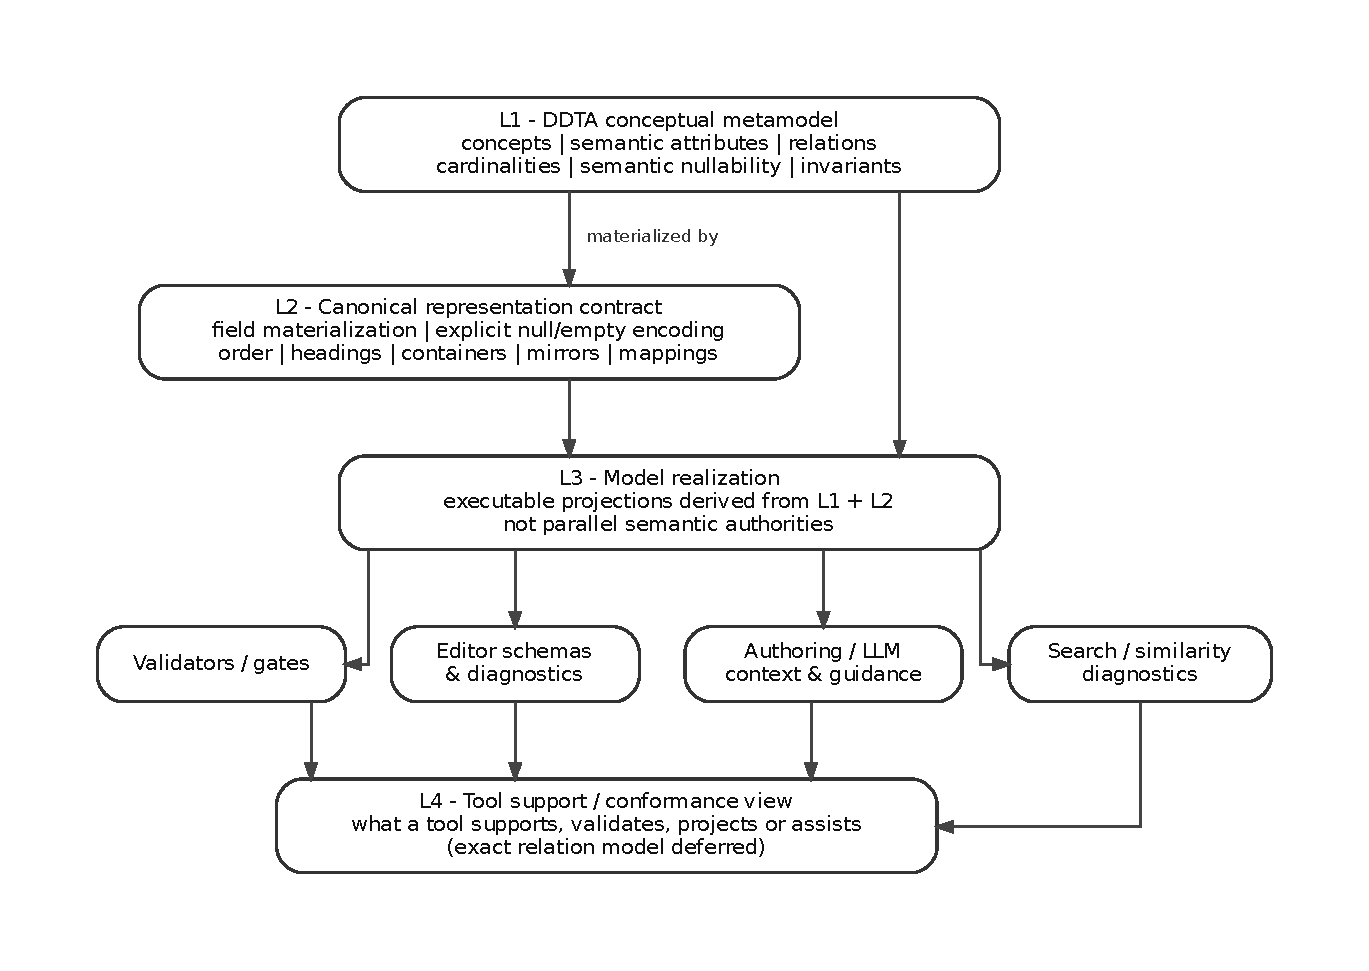
\includegraphics{../../00-foundations/01-model-layering/diagrams/MODEL_TO_EXECUTABLE_PROJECTIONS.pdf}
\caption{Model to executable projections}
\end{figure}

\subsection{Reading questions}\label{reading-questions}

When comparing each pair, ask:

\begin{enumerate}
\def\labelenumi{\arabic{enumi}.}
\tightlist
\item
  Does the revised Context identify a real \textbf{decision-local}
  problem rather than explain the whole parent MR?
\item
  Is the Decision precise about the choice without becoming its complete
  implementation specification?
\item
  Does the wording preserve the correct semantic owner: DDTA/metamodel,
  governed project, ThreatForge tool, or ThreatForge project operations?
\item
  If ThreatForge were replaced by another tool, would a statement that
  should remain true still be owned by DDTA rather than by the tool?
\item
  Are persistent/cross-cutting rules preserved as governed intent
  without adding ad-hoc fields such as \texttt{applicability},
  \texttt{vocabulary} or \texttt{patterns}?
\item
  Does \texttt{Consequences} expose the important trade-offs of the
  choice?
\item
  Does the redistribution note move only independently checkable
  obligations/planning downstream, or has it accidentally discarded part
  of the choice?
\item
  When a revised ADR mentions a canonical model, contract, projection,
  validator or editor behavior, does it preserve one semantic authority
  and let representation/executable detail derive downstream?
\item
  Could the decision eventually survive a change of programmer/LLM
  through a future governed effective-context/coverage mechanism rather
  than human memory?
\end{enumerate}

\subsection{Two concrete cross-document evidence cases
retained}\label{two-concrete-cross-document-evidence-cases-retained}

\begin{itemize}
\tightlist
\item
  \textbf{ADR-0002 Vocabulary} exposes a failure mode in the current
  ThreatForge decomposition: the Decision and canonical vocabulary still
  exist, but the MR-0001 Requirement registry has no Requirement
  directly owned by ADR-0002; current vocabulary tooling is instead
  governed through later ADR-0004 Requirements. Persistent intent can
  therefore become less explicit even when artifacts survive.
\item
  \textbf{ADR-0006 Handoff} is a positive counterexample: it has
  dedicated downstream Functional/Governance Requirements, including
  explicit continuity for a new LLM/session. It demonstrates how an
  operational Decision can remain connected to verifiable downstream
  obligations.
\end{itemize}

These cases constrain the \textbf{overall documentation model}; they are
not reasons to add vocabulary- or handoff-specific fields to
\texttt{Decision}.

\newpage

\section{MR-0001 - Gestione documentale
governata}\label{mr-0001---gestione-documentale-governata}

\subsection{MR-0001 / ADR-0001 - Adozione del Diátaxis framework per la
classificazione
documentale}\label{mr-0001-adr-0001---adozione-del-diuxe1taxis-framework-per-la-classificazione-documentale}

\subsubsection{Historical ADR semantic
body}\label{historical-adr-semantic-body}

\paragraph{Context}\label{context}

La documentazione ThreatForge distingue documenti scritti per
apprendere, eseguire un compito, consultare un riferimento o comprendere
il modello.

Senza una classificazione documentale esplicita, tutorial, how-to guide,
reference ed explanation possono essere confusi. Questa confusione rende
incerta l'autorità del contenuto e può portare a usare spiegazioni come
se fossero sorgenti normative.

\paragraph{Decision}\label{decision}

ThreatForge adotta il Diátaxis framework come modello di classificazione
documentale.

Le categorie documentali Diátaxis sono:

\begin{itemize}
\tightlist
\item
  tutorial;
\item
  how-to guide;
\item
  reference;
\item
  explanation.
\end{itemize}

Nel modello ThreatForge:

\begin{itemize}
\tightlist
\item
  i documenti \texttt{tutorial} guidano l'apprendimento progressivo;
\item
  i documenti \texttt{how-to} guidano azioni operative;
\item
  i documenti \texttt{reference} descrivono sorgenti consultabili e
  includono materiale normativo quando sono collegati a
  Macro-requirement, Decision, Requirement, registri, grafi o controlli;
\item
  i documenti \texttt{explanation} chiariscono il modello per persone e
  LLM, senza costituire fonte canonica di Requirement, registry, schema,
  procedure verificabili o controlli deterministici.
\end{itemize}

Diátaxis classifica la funzione del documento e non sostituisce
registri, grafi, Requirement, asset registry, vocabolari controllati o
controlli deterministici.

La decisione comprende l'uso di Diátaxis come classificazione
documentale, la distinzione tra le quattro categorie e la separazione
tra documentazione normativa e documentazione esplicativa. I Requirement
derivati applicano questa classificazione ai documenti governati.

\paragraph{Consequences}\label{consequences}

\begin{itemize}
\tightlist
\item
  Benefit: La documentazione acquisisce una classificazione
  comprensibile e stabile.
\item
  Benefit: I documenti esplicativi restano distinti dalle sorgenti
  normative.
\item
  Benefit: I documenti di riferimento rimangono precisi e controllabili.
\item
  Benefit: Programmatori, persone non tecniche, LLM e controlli
  deterministici distinguono il ruolo previsto di ogni documento.
\item
  Cost: La categoria Diátaxis richiede una fonte canonica unica
  governata separatamente.
\item
  Risk: Diátaxis può essere applicato in modo errato quando viene
  trattato come semplice struttura di cartelle anziché come
  classificazione basata sul bisogno del lettore.
\item
  Cost: La distinzione tra \texttt{reference} ed \texttt{explanation}
  richiede revisione editoriale oltre al controllo automatico.
\item
  Constraint: La classificazione Diátaxis non sostituisce le altre fonti
  canoniche e i controlli governati.
\end{itemize}

\paragraph{Non-goals}\label{non-goals}

\begin{itemize}
\tightlist
\item
  Definire la fonte canonica della categoria Diátaxis
\item
  Definire la convenzione dei percorsi documentali
\item
  Definire i campi minimi del frontmatter documentale
\item
  Definire il ciclo di vita documentale
\item
  Definire la generazione del libro PDF o delle viste HTML
\item
  Definire tutti i controlli deterministici della documentazione
\item
  Introdurre RDF, SKOS, SHACL o OWL come formato obbligatorio
\end{itemize}

\subsubsection{Revised candidate ADR}\label{revised-candidate-adr}

\paragraph{Revised title}\label{revised-title}

Diátaxis come classificazione comune della funzione documentale

\paragraph{Context}\label{context-1}

Un metodo di documentazione governata applicato a progetti diversi deve
permettere a lettori, programmatori, strumenti e LLM di riconoscere
rapidamente \textbf{per quale bisogno di lettura} esiste un documento.
Lasciare a ogni progetto una classificazione proprietaria aumenta il
costo di apprendimento e rende meno trasferibile l'esperienza maturata
tra progetti.

Occorre quindi scegliere se il metodo documentale adotti una
classificazione condivisa e riconoscibile oppure lasci che ogni progetto
inventi autonomamente la propria organizzazione funzionale.

\paragraph{Decision}\label{decision-1}

Il metodo DDTA adotta \textbf{Diátaxis} come classificazione comune
della funzione editoriale dei documenti, distinguendo \texttt{tutorial},
\texttt{how-to\ guide}, \texttt{reference} ed \texttt{explanation}
secondo il bisogno del lettore.

La classificazione editoriale non determina da sola l'autorità semantica
del contenuto: l'autorità continua a dipendere dal modello documentale
governato e dalle fonti che possiedono l'informazione.

\paragraph{Consequences}\label{consequences-1}

\begin{itemize}
\tightlist
\item
  Benefit: progetti governati diversi possono condividere
  un'organizzazione leggibile senza una tassonomia proprietaria per
  progetto.
\item
  Benefit: nuovi lettori e agenti possono riusare conoscenza precedente
  su come orientarsi nella documentazione.
\item
  Cost: la corretta classificazione richiede giudizio editoriale e non
  puo essere ridotta alla sola posizione del file.
\item
  Risk: Diátaxis puo essere degradato a convenzione di cartelle perdendo
  il legame con il bisogno del lettore.
\end{itemize}

\subsubsection{Redistribution / ownership
notes}\label{redistribution-ownership-notes}

\begin{itemize}
\tightlist
\item
  \textbf{Ownership candidate: DDTA method}, non ThreatForge tool. Se
  accettata definitivamente, questa scelta deve vivere nella specifica
  del metodo e ThreatForge deve soltanto supportarla.
\item
  Template, rappresentazione, assistenza di authoring e controlli sono
  downstream e non definiscono il significato della classificazione.
\item
  Le vecchie liste di Non-goals non vengono ripetute: una falsa
  interpretazione va corretta in \texttt{Context\ +\ Decision}, non
  patchata con esclusioni.
\end{itemize}

\subsection{MR-0001 / ADR-0002 - Vocabolario controllato della
documentazione
governata}\label{mr-0001-adr-0002---vocabolario-controllato-della-documentazione-governata}

\subsubsection{Historical ADR semantic
body}\label{historical-adr-semantic-body-1}

\paragraph{Context}\label{context-2}

La documentazione governata usa termini ricorrenti come
Macro-requirement, Decision, Requirement, registro, asset, fonte
canonica e output derivato.

Quando questi termini restano liberi, documenti diversi possono usare
sinonimi o significati divergenti. Il corpus diventa meno leggibile per
persone, sviluppatori e LLM e più difficile da sottoporre a controlli
deterministici.

\paragraph{Decision}\label{decision-2}

ThreatForge adotta un vocabolario controllato minimo per i termini della
documentazione governata.

Il vocabolario controllato costituisce la fonte canonica dei termini
documentali centrali. Ogni termine contiene almeno:

\begin{itemize}
\tightlist
\item
  identificativo stabile;
\item
  nome canonico;
\item
  stato;
\item
  definizione sintetica.
\end{itemize}

Il vocabolario rappresenta anche label controllate con ruolo esplicito,
lingua, ragione d'uso, alias ammessi, traduzioni, label candidate e
label vietate.

Il registro governato del vocabolario risiede nel percorso logico:

\begin{Shaded}
\begin{Highlighting}[]
\NormalTok{docs/reference/project{-}model/registers/vocabularies/documentation{-}terms.registry.yml}
\end{Highlighting}
\end{Shaded}

Il testo normativo privilegia i termini presenti nel vocabolario
controllato. Un termine di dominio non ancora registrato entra nel
processo come candidato da valutare, anziché come sinonimo libero.

La decisione comprende l'esistenza del vocabolario, il suo ruolo di
fonte canonica, il percorso iniziale del registro e la base per future
metriche deterministiche di qualità terminologica. Gli incrementi
derivati applicano il vocabolario ai documenti governati e separano le
decisioni sulle metriche di qualità e sul registro asset.

\paragraph{Consequences}\label{consequences-2}

\begin{itemize}
\tightlist
\item
  Benefit: I termini centrali della documentazione hanno una fonte
  canonica.
\item
  Benefit: I sinonimi liberi diventano rilevabili e discutibili.
\item
  Benefit: Persone, sviluppatori e LLM dispongono di un riferimento
  esplicito per interpretare il corpus documentale.
\item
  Benefit: I futuri report di qualità possono confrontare i documenti
  con un registro controllato.
\item
  Cost: Il vocabolario richiede manutenzione e disciplina editoriale.
\item
  Risk: Un vocabolario troppo ampio può diventare rumoroso e poco utile.
\item
  Risk: Un vocabolario troppo piccolo può lasciare ambiguità e sinonimi
  non governati.
\item
  Constraint: Le label utili alla leggibilità non creano fonti canoniche
  alternative.
\end{itemize}

\paragraph{Non-goals}\label{non-goals-1}

\begin{itemize}
\tightlist
\item
  Definire tutte le tassonomie del progetto
\item
  Definire il registro asset
\item
  Definire formule, soglie o gate di qualità del corpus
\item
  Definire algoritmi di term extraction
\item
  Adottare RDF, SKOS, SHACL o OWL come formato obbligatorio
\item
  Implementare tool o controlli automatici
\end{itemize}

\subsubsection{Revised candidate ADR}\label{revised-candidate-adr-1}

\paragraph{Revised title}\label{revised-title-1}

Vocabolario governato come fonte unica del linguaggio condiviso

\paragraph{Context}\label{context-3}

La documentazione governata usa concetti che devono mantenere
significato coerente attraverso documenti, progetti, sessioni e agenti
differenti. Se definizioni e sinonimi vengono ricostruiti localmente, il
corpus puo divergere semanticamente anche quando ogni singolo documento
resta formalmente valido.

Occorre quindi scegliere se il significato dei termini condivisi dipenda
dalla memoria e dalle convenzioni locali oppure sia governato da una
fonte comune.

\paragraph{Decision}\label{decision-3}

Il metodo DDTA governa i termini condivisi attraverso \textbf{una fonte
unica di vocabolario controllato}. Le definizioni comuni vengono
referenziate o risolte dalla loro fonte governata e non copiate
cumulativamente nei documenti discendenti.

Termini specifici di un dominio o di una parte del progetto possono
essere aggiunti quando necessari senza ridefinire implicitamente i
termini condivisi e senza creare proprietari concorrenti dello stesso
significato.

\paragraph{Consequences}\label{consequences-3}

\begin{itemize}
\tightlist
\item
  Benefit: persone, strumenti e LLM possono ricostruire il significato
  dei termini senza dipendere dal contesto ricordato da una sessione
  precedente.
\item
  Benefit: una modifica terminologica ha un proprietario governato
  invece di richiedere copie sincronizzate in molti documenti.
\item
  Cost: il metodo deve rendere il vocabolario rilevante effettivamente
  recuperabile durante authoring e review.
\item
  Risk: una fonte canonica che esiste ma non viene propagata ai consumer
  puo sopravvivere formalmente senza influenzare il lavoro reale.
\end{itemize}

\subsubsection{Redistribution / ownership
notes}\label{redistribution-ownership-notes-1}

\begin{itemize}
\tightlist
\item
  \textbf{Ownership candidate: DDTA method / cross-document governance},
  non ThreatForge tool.
\item
  Schema delle entry, label, traduzioni, path e checker sono scelte
  downstream.
\item
  Il failure mode ThreatForge resta evidenza: ADR-0002 non ha una catena
  Requirement diretta nel baseline mentre il vocabolario continua a
  essere consumato da tooling successivo.
\item
  Il meccanismo per rendere il vocabolario effettivamente disponibile ai
  discendenti resta \textbf{OPEN}: non viene risolto aggiungendo campi
  duplicati a MR/ADR/REQ.
\end{itemize}

\subsection{MR-0001 / ADR-0003 - Tracciabilità degli artefatti
implementativi previsti e
realizzati}\label{mr-0001-adr-0003---tracciabilituxe0-degli-artefatti-implementativi-previsti-e-realizzati}

\subsubsection{Historical ADR semantic
body}\label{historical-adr-semantic-body-2}

\paragraph{Context}\label{context-4}

La documentazione governata può citare tool, report, gate, fixture o
altri artefatti implementativi collegati alla soddisfazione dei
Requirement.

Quando questi artefatti compaiono soltanto nella prosa di Decision,
Requirement o how-to guide, risultano difficili da controllare
deterministicamente. Possono essere dimenticati, rimanere incompleti o
divergere dal codice realmente scritto.

Il progetto necessita di una fonte controllata che colleghi Requirement,
artefatti previsti, artefatti implementati, percorsi, comandi di
verifica e stato di completamento.

La tracciabilità copre sia il lavoro già implementato sia il lavoro
pianificato ma non ancora realizzato.

\paragraph{Decision}\label{decision-4}

ThreatForge usa un implementation trace registry per rappresentare gli
artefatti implementativi collegati ai Requirement.

Il registro include artefatti pianificati e artefatti implementati.

Ogni artefatto pianificato contiene almeno:

\begin{itemize}
\tightlist
\item
  identificativo governato;
\item
  tipo di artefatto;
\item
  stato;
\item
  Requirement collegati;
\item
  percorso previsto;
\item
  ragione;
\item
  condizione di completamento.
\end{itemize}

Ogni artefatto implementato contiene almeno:

\begin{itemize}
\tightlist
\item
  identificativo governato;
\item
  tipo di artefatto;
\item
  stato;
\item
  Requirement collegati;
\item
  percorso implementato;
\item
  eventuale comando di verifica.
\end{itemize}

Gli artefatti pianificati e non ancora implementati producono un warning
deterministico. Gli artefatti dichiarati come implementati sono
confrontati deterministicamente con l'esistenza dei Requirement
collegati, l'esistenza del percorso implementato, la coerenza tra
registro e dichiarazioni di tracciabilità nel codice e l'assenza di
riferimenti a Requirement inesistenti.

Il registro non sostituisce i Requirement. Il body del Requirement
descrive l'obbligo; l'implementation trace registry descrive gli
artefatti previsti o realizzati per soddisfarlo.

La decisione copre tool, report, gate, fixture, artefatti di verifica e
altri artefatti implementativi collegati ai Requirement. La sequenza di
adozione comprende il Requirement funzionale del registro, il Governance
Requirement per il controllo di coerenza, il primo registro minimo e il
checker dei warning sugli artefatti pianificati non completati.

\paragraph{Consequences}\label{consequences-4}

\begin{itemize}
\tightlist
\item
  Benefit: Le promesse implementative non restano soltanto nella prosa
  della documentazione governata.
\item
  Benefit: Gli artefatti pianificati diventano visibili tramite warning
  deterministici.
\item
  Benefit: La coerenza tra Requirement, registro e codice è
  controllabile senza leggere manualmente tutti i body.
\item
  Benefit: Il registro distingue lavoro pianificato, lavoro implementato
  e lavoro da completare.
\item
  Benefit: Le future relazioni di grafo possono derivare da Requirement,
  implementation trace registry e dichiarazioni nel codice.
\item
  Cost: Il registro richiede sincronizzazione continua con Requirement e
  codice.
\item
  Risk: Un registro non aggiornato può introdurre falsi warning o falsa
  sicurezza.
\item
  Cost: La disciplina iniziale aumenta la verbosità prima
  dell'automazione completa.
\item
  Risk: Warning non calibrati sugli artefatti pianificati possono
  diventare rumore ignorato.
\end{itemize}

\paragraph{Non-goals}\label{non-goals-2}

\begin{itemize}
\tightlist
\item
  Definire il formato definitivo dello schema del registro
\item
  Definire tutti i valori controllati ammessi
\item
  Implementare il tool di validazione nella decisione stessa
\item
  Definire soglie di qualità del corpus documentale
\item
  Definire il modello completo di generazione del grafo
\end{itemize}

\subsubsection{Revised candidate ADR}\label{revised-candidate-adr-2}

\paragraph{Revised title}\label{revised-title-2}

Supporto ThreatForge alla tracciabilità della realizzazione governata

\paragraph{Context}\label{context-5}

I progetti governati possono aver bisogno di rendere osservabile come un
obbligo documentato viene pianificato, realizzato e verificato
attraverso artefatti differenti. ThreatForge deve poter supportare
questa conoscenza senza trasformare la propria implementazione nella
fonte del significato dell'obbligo o della relazione prevista dal
modello.

Occorre quindi decidere come il tool supporti la tracciabilità della
realizzazione mantenendo separata la semantica governata del progetto.

\paragraph{Decision}\label{decision-5}

ThreatForge supporta una \textbf{tracciabilità implementativa governata}
consumando le identità, le relazioni e le regole esposte dal modello del
progetto e collegandole alle evidenze o agli artefatti di realizzazione
gestiti dal tool.

ThreatForge non rende vero un obbligo per il solo fatto di registrare un
artefatto e non definisce autonomamente che cosa significhi soddisfare
l'obbligo: la semantica resta posseduta dal modello governato, mentre il
tool rende la relazione osservabile, interrogabile e verificabile
secondo quel contratto.

\paragraph{Consequences}\label{consequences-5}

\begin{itemize}
\tightlist
\item
  Benefit: la conoscenza sulla realizzazione puo essere automatizzata
  senza spostare l'autorita semantica nel tool.
\item
  Benefit: il tool puo distinguere pianificazione, realizzazione ed
  evidenza quando tali distinzioni sono previste dal modello.
\item
  Cost: ThreatForge deve restare allineato alle relazioni e ai contratti
  del modello che supporta.
\item
  Risk: se il tool introduce stati o significati non previsti dal
  modello, diventa una fonte semantica concorrente.
\end{itemize}

\subsubsection{Redistribution / ownership
notes}\label{redistribution-ownership-notes-2}

\begin{itemize}
\tightlist
\item
  \textbf{Ownership split detected.} La necessita e la semantica
  generale della tracciabilita sono questioni del DDTA/metamodello;
  questa ADR puo legittimamente decidere solo \textbf{come ThreatForge
  le supporta}.
\item
  Il termine di classe \texttt{Requirement} viene evitato nella
  candidata finche il relativo modello non e chiuso.
\item
  Registry, stati, warning, checker, campi e cardinalita sono
  downstream/tool design.
\end{itemize}

\subsection{MR-0001 / ADR-0004 - Modello di label controllate e valori
tassonomici
documentali}\label{mr-0001-adr-0004---modello-di-label-controllate-e-valori-tassonomici-documentali}

\subsubsection{Historical ADR semantic
body}\label{historical-adr-semantic-body-3}

\paragraph{Context}\label{context-6}

Il vocabolario controllato introdotto da ADR-0002 richiede una
distinzione più precisa tra termine canonico, alias ammesso, traduzione,
label storica, label candidata e label vietata.

Un campo generico come \texttt{allowed\_labels} è troppo permissivo: può
mescolare sinonimi, acronimi, traduzioni, nomi storici, varianti
operative e label di visualizzazione. Questa ambiguità rende difficile
stabilire quale forma sia canonica, quale sia soltanto leggibile, quale
sia accettata per compatibilità e quale sia segnalata dai controlli.

La documentazione governata usa anche campi ricorrenti come
\texttt{status}, \texttt{artifact\_type}, \texttt{requirement\_type},
\texttt{decision\_type}, \texttt{check\_status} e ruoli delle label.
Stringhe libere in questi campi consentono a registri diversi di usare
valori simili con significati differenti.

Il caso più rischioso è \texttt{status}: valori come \texttt{active},
\texttt{draft}, \texttt{implemented} o \texttt{deprecated} non hanno un
significato universale. Il significato cambia in base al registro e al
tipo di record. Un check \texttt{active} viene eseguito
dall'orchestratore; un termine \texttt{active} è utilizzabile nel
vocabolario; una Decision \texttt{accepted} è applicabile; un artefatto
\texttt{implemented} esiste ed è verificabile. Una tassonomia globale di
\texttt{status} risulterebbe ambigua.

I nomi temporanei usati per organizzare il lavoro non appartengono ai
concetti canonici del modello documentale. Restano utilizzabili nei path
tecnici o nelle procedure operative senza diventare termini di dominio
nella documentazione governata.

\paragraph{Decision}\label{decision-6}

Il vocabolario controllato rappresenta le label tramite un modello
esplicito basato su ruolo, lingua e ragione d'uso.

Ogni termine governato mantiene un solo \texttt{canonical\_name} e una
\texttt{canonical\_language}. Ogni label associata a un termine dichiara
almeno:

\begin{itemize}
\tightlist
\item
  \texttt{value};
\item
  \texttt{language};
\item
  \texttt{role};
\item
  \texttt{reason}.
\end{itemize}

I ruoli iniziali delle label sono:

\begin{itemize}
\tightlist
\item
  \texttt{preferred}: forma preferita nella documentazione governata;
\item
  \texttt{accepted\_alias}: alias ammesso per una ragione esplicita,
  come un acronimo tecnico o una compatibilità storica;
\item
  \texttt{translation}: traduzione leggibile e non canonica;
\item
  \texttt{forbidden}: forma vietata e segnalabile;
\item
  \texttt{candidate}: forma proposta e non ancora accettata;
\item
  \texttt{historical}: forma storica riconoscibile e non preferita per
  nuovo testo.
\end{itemize}

Un sinonimo non costituisce automaticamente una label ammessa. Ogni
alias accettato conserva una ragione esplicita. Le traduzioni supportano
la lettura senza creare una seconda fonte canonica. Le label vietate e
le frasi temporanee da evitare sono registrate esplicitamente per
consentire segnalazioni deterministiche.

I campi documentali e di registro con valori ripetuti evolvono verso
value set tassonomici contestuali. Ogni value set dichiara almeno:

\begin{itemize}
\tightlist
\item
  \texttt{name};
\item
  \texttt{field\_name};
\item
  \texttt{applies\_to\_registry};
\item
  \texttt{applies\_to\_record};
\item
  \texttt{status} del value set;
\item
  \texttt{description};
\item
  lista dei valori ammessi con \texttt{value} e \texttt{meaning}.
\end{itemize}

Non esiste una tassonomia globale generica per \texttt{status} quando lo
stesso valore assume significati differenti in registri diversi. I
valori controllati sono specifici del contesto, tra cui
\texttt{check\_status}, \texttt{implementation\_artifact\_status},
\texttt{decision\_status}, \texttt{requirement\_lifecycle\_status},
\texttt{vocabulary\_term\_status} e \texttt{field\_value\_set\_status}.

Lo stato di un Requirement resta distinto dallo stato di
implementazione. Il lifecycle di un Requirement comprende
\texttt{draft}, \texttt{accepted}, \texttt{superseded},
\texttt{deprecated} e \texttt{removed}; lo stato implementativo deriva
dalla tracciabilità e dalle verifiche anziché dal medesimo campo
\texttt{status}.

Il campo \texttt{requirement\_type} contiene esclusivamente tipi
concreti registrati nel proprio value set contestuale.
\texttt{specialized} rappresenta una categoria astratta e non compare
come valore del campo né come alias di un tipo concreto.

Ogni tipo concreto dichiara, oltre a \texttt{value} e \texttt{meaning},
l'eventuale appartenenza alla categoria specializzata, la presenza di un
Requirement padre e i tipi concreti ammessi come padre. I tipi concreti
disponibili sono esclusivamente quelli registrati nel value set
contestuale \texttt{requirement\_type} e associati alle rispettive
varianti e regole canoniche. Ogni nuovo tipo entra attraverso
un'estensione governata esplicita e non attraverso una lista locale o un
alias implicito.

La decisione comprende la sostituzione di \texttt{allowed\_labels}, la
distinzione dei ruoli delle label, i value set contestuali, la
scomposizione di \texttt{status} e l'esclusione dei nomi temporanei dai
concetti canonici. Gli incrementi derivati aggiornano il registro del
vocabolario, definiscono i primi value set, introducono il Governance
Requirement di coerenza e aggiungono il controllo sulle label e sui
valori fuori contesto.

\paragraph{Consequences}\label{consequences-6}

\begin{itemize}
\tightlist
\item
  Benefit: Il vocabolario riduce l'ambiguità tra forme canoniche,
  sinonimi, traduzioni e acronimi.
\item
  Benefit: Le label ammesse conservano una ragione esplicita.
\item
  Benefit: Le traduzioni migliorano la leggibilità senza diventare fonti
  canoniche.
\item
  Benefit: I controlli futuri distinguono errori, warning e candidati.
\item
  Benefit: I valori dei campi ricorrenti diventano verificabili nel
  proprio contesto.
\item
  Benefit: Il campo \texttt{status} non viene trattato come una lista
  globale ambigua.
\item
  Benefit: Ogni valore controllato conserva un significato adatto al
  registro e al record di applicazione.
\item
  Cost: Il registro del vocabolario diventa più verboso.
\item
  Cost: Il registro dei valori tassonomici richiede più record.
\item
  Cost: La classificazione delle label richiede disciplina editoriale.
\item
  Cost: I tool di validazione gestiscono più campi e più contesti.
\item
  Risk: Una label utile alla lettura può sembrare canonica quando il
  ruolo non è classificato correttamente.
\end{itemize}

\paragraph{Non-goals}\label{non-goals-3}

\begin{itemize}
\tightlist
\item
  Definire tutte le tassonomie del progetto
\item
  Implementare il controllo terminologico completo sul corpus nella
  decisione stessa
\item
  Definire metriche di qualità del corpus
\item
  Definire il registro asset
\item
  Decidere il modello completo di implementation state derivato
\end{itemize}

\subsubsection{Revised candidate ADR}\label{revised-candidate-adr-3}

\paragraph{Revised title}\label{revised-title-3}

Risoluzione contestuale dei valori controllati da fonti governate

\paragraph{Context}\label{context-7}

ThreatForge consuma campi e label controllati definiti dalla
documentazione governata. Se il tool codifica enum globali o interpreta
autonomamente stringhe come \texttt{status}, puo attribuire significati
diversi da quelli previsti dal modello o dal contesto documentale.

Occorre quindi decidere se i consumer ThreatForge mantengano inventari
locali oppure risolvano significati e valori dalle fonti governate che
li possiedono.

\paragraph{Decision}\label{decision-7}

ThreatForge risolve \textbf{label e valori controllati nel loro contesto
governato} e deriva gli inventari dai cataloghi o contratti del
modello/progetto anziche mantenere enum semantici concorrenti nel codice
dei consumer.

Il tool puo validare che un valore sia ammesso nel contesto dichiarato,
ma non introduce autonomamente una semantica universale di
\texttt{status}, lifecycle o tipo documentale.

\paragraph{Consequences}\label{consequences-7}

\begin{itemize}
\tightlist
\item
  Benefit: consumer differenti possono usare gli stessi significati
  senza duplicare liste locali.
\item
  Benefit: l'evoluzione del modello non richiede di reinterpretare
  manualmente gli stessi valori in ogni adapter.
\item
  Cost: resolution e provenance delle fonti controllate diventano
  dipendenze esplicite del tool.
\item
  Risk: cache o proiezioni obsolete possono applicare un significato non
  piu corrente.
\end{itemize}

\subsubsection{Redistribution / ownership
notes}\label{redistribution-ownership-notes-3}

\begin{itemize}
\tightlist
\item
  \textbf{Ownership candidate: ThreatForge tool support.} La semantica
  dei value set e dei lifecycle appartiene al modello/metodo che li
  definira.
\item
  L'ADR storica contiene anche decisioni generali su label, lifecycle e
  tipi di requisito che non devono essere fissate indirettamente dal
  tool.
\item
  Schema concreto, ruoli delle label e tassonomie restano fuori dal
  Decision metamodel corrente.
\end{itemize}

\subsection{MR-0001 / ADR-0006 - Handoff locale come artefatto governato
di continuità
operativa}\label{mr-0001-adr-0006---handoff-locale-come-artefatto-governato-di-continuituxe0-operativa}

\subsubsection{Historical ADR semantic
body}\label{historical-adr-semantic-body-4}

\paragraph{Context}\label{context-8}

Il lavoro governato può estendersi oltre una singola sessione operativa.
In questi casi un handoff riproducibile consente di riprendere il lavoro
senza dipendere dalla memoria della chat o da archivi prodotti
esternamente.

Lo ZIP di handoff nasce dal repository locale, che costituisce la fonte
canonica per stato, registri, check, comandi e contenuto del progetto.

Un handoff soltanto riassuntivo non offre sufficiente continuità per la
ripresa dello sviluppo da parte di un LLM: il modello necessita anche
dei file governati, del codice, dei contratti, dei test e degli altri
sorgenti tracciati.

\paragraph{Decision}\label{decision-8}

ThreatForge introduce un handoff archive locale come artefatto governato
di continuità operativa.

Un tool locale tracciato nell'implementation trace registry produce
l'archive. Il contenuto usa la label canonica di prodotto
\texttt{ThreatForge} e include esclusivamente il progetto operativo
corrente; gli artefatti legacy archiviati sotto \texttt{old/} restano
esclusi dallo snapshot di continuità.

L'archive include uno snapshot del progetto basato sui file tracciati da
Git, così che un LLM o un operatore possa leggere lo stato sorgente
necessario per riprendere lo sviluppo. Lo snapshot esclude
\texttt{.git}, dipendenze installate, cache, build output e artifact
generati non tracciati.

\paragraph{Consequences}\label{consequences-8}

\begin{itemize}
\tightlist
\item
  Benefit: L'handoff deriva dalla fonte canonica locale anziché dalla
  sandbox della chat.
\item
  Benefit: Lo stato del repository e l'output dei check vengono raccolti
  dal tool locale.
\item
  Benefit: L'archive supporta la continuazione in una nuova chat o la
  consegna del contesto a un operatore.
\item
  Cost: L'archive aumenta di dimensione perché contiene lo snapshot dei
  file tracciati.
\item
  Constraint: Il tool resta sotto MR-0001 perché impacchetta
  documentazione governata, registri, sorgenti tracciati e verifiche di
  continuità.
\item
  Constraint: Lo snapshot include soltanto il progetto operativo
  corrente e gli artefatti Git tracciati ammessi.
\end{itemize}

\subsubsection{Revised candidate ADR}\label{revised-candidate-adr-4}

\paragraph{Revised title}\label{revised-title-4}

Handoff governato per la continuità dello sviluppo ThreatForge

\paragraph{Context}\label{context-9}

Lo sviluppo di ThreatForge attraversa sessioni di lavoro, programmatori
e LLM differenti. Affidare la continuita alla memoria di una chat o a un
riassunto manuale rende facile perdere Decision, stato del repository,
verifiche e sorgenti necessarie a proseguire il lavoro in modo
riproducibile.

Occorre quindi decidere se la continuita operativa dello sviluppo
ThreatForge resti una pratica informale oppure venga resa ricostruibile
a partire dallo stato governato del progetto.

\paragraph{Decision}\label{decision-9}

Il processo di sviluppo di ThreatForge usa un \textbf{handoff governato
e ricostruibile} derivato dallo stato canonico del repository e dalle
evidenze operative necessarie a riprendere il lavoro.

L'handoff non sostituisce le fonti governate e non rende canonico il
riassunto della sessione: serve a trasportare abbastanza contesto e
sorgenti per consentire al nuovo agente di verificare e ricostruire lo
stato rilevante.

\paragraph{Consequences}\label{consequences-9}

\begin{itemize}
\tightlist
\item
  Benefit: il cambio di sessione o agente non dipende dalla memoria
  dell'operatore precedente.
\item
  Benefit: la continuita viene verificata rispetto allo stato del
  progetto, non rispetto a una narrazione isolata.
\item
  Cost: l'handoff deve essere mantenuto riproducibile e sufficientemente
  completo.
\item
  Risk: un handoff incompleto o obsoleto puo dare falsa confidenza sulla
  continuita.
\end{itemize}

\subsubsection{Redistribution / ownership
notes}\label{redistribution-ownership-notes-4}

\begin{itemize}
\tightlist
\item
  \textbf{Ownership candidate: ThreatForge project operations}, non
  regola universale DDTA e non semantica del tool verso i target
  project.
\item
  Il caso resta importante per la tesi come evidenza pratica di
  \texttt{recoverability} e perdita di contesto tra agenti.
\item
  ZIP, manifest, snapshot, dry-run e filtri sono downstream operational
  requirements/implementation.
\end{itemize}

\subsection{MR-0001 / ADR-0007 - Canonical document models and
model-oriented
validation}\label{mr-0001-adr-0007---canonical-document-models-and-model-oriented-validation}

\subsubsection{Historical ADR semantic
body}\label{historical-adr-semantic-body-5}

\paragraph{Context}\label{context-10}

ThreatForge governs Macro-requirements, decisions and requirements
through YAML registry records and Markdown bodies. Existing checks
validate selected fragments of those representations, but the structural
rules are distributed across independent tools and do not yet form an
explicit document model.

The governed corpus also contains inconsistent headings, languages,
punctuation and normative forms. Live authoring assistance,
deterministic migration and reliable LLM analysis require one canonical
description of each document model and stable diagnostics shared by
gates and editors.

\paragraph{Decision}\label{decision-10}

ThreatForge defines governed document models through the canonical
document model index. Each active model entry references exactly one
YAML registry profile and exactly one Markdown body profile, and the
profiles referenced by active model entries form the active
representation-profile inventory. This Decision does not impose a fixed
number of models or profiles.

Canonical model definitions are organized by model and representation. A
shared validation engine consumes those definitions, while one
entrypoint validates each complete logical model and one cross-model
entrypoint validates relationships among models.

Model checkers absorb overlapping partial document checks after
equivalent rule coverage is proven. Every diagnostic uses a stable rule
identifier that is shared by repository gates, migration reports, editor
diagnostics, quick fixes and deterministic fixtures.

Canonical identifiers, YAML field names, Markdown headings and persisted
controlled values are English. Future translations are presentation
metadata and do not create alternative canonical identifiers or values.

New model checks are introduced as non-blocking planned checks. They
become active only after every active registry record and referenced
body has been migrated and the complete model report contains no errors.
ThreatForge does not retain a legacy validation mode for the previous
body formats.

\paragraph{Consequences}\label{consequences-10}

\begin{itemize}
\tightlist
\item
  Benefit: The complete rule set for one document type is discoverable
  from one logical model.
\item
  Benefit: Repository gates, VS Code and the future web editor can use
  identical rule identifiers and semantics.
\item
  Cost: Existing governed records and bodies require a reviewed
  repository-wide migration.
\item
  Risk: Activating model checks before migration would make the governed
  repository gate fail.
\item
  Constraint: Partial checks may be removed only after the replacement
  model checker proves equivalent or stronger coverage.
\end{itemize}

\paragraph{Non-goals}\label{non-goals-4}

\begin{itemize}
\tightlist
\item
  Immediate implementation of the validation engine
\item
  Immediate activation of new blocking checks
\item
  Governance of ordinary Diátaxis documentation as governed document
  models
\end{itemize}

\subsubsection{Revised candidate ADR}\label{revised-candidate-adr-5}

\paragraph{Revised title}\label{revised-title-5}

Contratti eseguibili dei modelli documentali consumati da ThreatForge

\paragraph{Context}\label{context-11}

Validatori, editor, generatori e migrazioni ThreatForge devono
interpretare gli stessi modelli documentali. Se ogni consumer
ricostruisce autonomamente struttura, campi e regole, il tool puo
produrre comportamenti divergenti e finire per ridefinire implicitamente
il modello che dovrebbe soltanto supportare.

Occorre quindi decidere come ThreatForge consumi in modo uniforme la
descrizione governata dei modelli documentali.

\paragraph{Decision}\label{decision-11}

ThreatForge usa \textbf{contratti eseguibili o proiezioni canoniche dei
modelli documentali governati} come fonte comune per validazione,
authoring, migrazione e altri consumer. I consumer derivano le proprie
regole da tali contratti anziche mantenere descrizioni semantiche locali
concorrenti.

Il contratto eseguibile e una rappresentazione consumabile dal tool: non
rende ThreatForge proprietario della semantica generale del documento,
che resta definita dal modello DDTA e dalle estensioni governate del
progetto.

\paragraph{Consequences}\label{consequences-11}

\begin{itemize}
\tightlist
\item
  Benefit: consumer differenti possono condividere interpretazione e
  diagnostica senza duplicare il modello nel codice.
\item
  Benefit: l'evoluzione del modello puo essere propagata attraverso una
  fonte consumabile comune.
\item
  Cost: i contratti devono restare tracciabili alla fonte semantica che
  rappresentano.
\item
  Risk: una proiezione obsoleta o arricchita con semantica
  tool-specifica puo diventare una fonte concorrente.
\end{itemize}

\subsubsection{Redistribution / ownership
notes}\label{redistribution-ownership-notes-5}

\begin{itemize}
\tightlist
\item
  \textbf{Ownership candidate: ThreatForge tool architecture.} Il tool
  possiede il modo in cui consuma il modello, non il significato
  generale dei tipi documentali.
\item
  Cardinalita dei profili, lingua dei campi, activation sequence e
  migrazione sono downstream.
\item
  Il rapporto esatto tra metamodello semantico e contratto eseguibile
  resta da definire nella futura mapping/serialization phase.
\end{itemize}

\subsection{MR-0001 / ADR-0008 - Canonical governed entity references in
Markdown
bodies}\label{mr-0001-adr-0008---canonical-governed-entity-references-in-markdown-bodies}

\subsubsection{Historical ADR semantic
body}\label{historical-adr-semantic-body-6}

\paragraph{Context}\label{context-12}

Governed Markdown bodies currently represent document identity in their
headers and controlled values in profile-defined sections, but they lack
one canonical representation for references to other governed entities.

Base Analysis Elements introduce the first immediate use case. The same
problem also applies to future threats, findings, mitigations, snapshots
and other canonical records. Free-form alternatives such as bare
identifiers, parenthesized tokens, Markdown links or independently
authored labels create ambiguous parsing and allow readable titles to
diverge from their authoritative records.

A reference also has different semantics from an origin relation. Text
containing an identifier does not establish when or why the referenced
entity came into existence.

\paragraph{Decision}\label{decision-12}

ThreatForge adopts one canonical governed entity reference payload:

\texttt{{[}\textless{}canonical-id\textgreater{}{]}\ \textless{}canonical-title\textgreater{}}

The canonical identifier is authoritative. The canonical title is a
required human-readable mirror resolved from the entity's authoritative
governed source. Exactly one ASCII space separates the closing bracket
from the title, and the payload contains no surrounding whitespace.

The containing body profile defines the reference-bearing position and
any Markdown container outside the payload. A list marker, section
heading or other profile-owned structure is not part of the reference
payload. Identical text outside a declared reference-bearing position
remains ordinary Markdown prose.

Each referenceable governed entity type is associated with one
registered canonical resolver. The resolver identifies the authoritative
source, canonical title, entity type and semantic eligibility rules for
the current document and reference position.

A canonical reference resolves to exactly one existing entity of an
allowed type. Unknown identifiers, ambiguous identifiers, disallowed
entity types, divergent titles and failed eligibility rules are invalid
reference states.

Alternative forms such as \texttt{(@BAE-0001)\ Title}, a bare
\texttt{BAE-0001}, or \texttt{{[}BAE-0001{]}(target)} are not canonical
governed entity references and receive no compatibility alias.

A textual reference does not create, originate or justify the referenced
entity. Origin, provenance, lifecycle and reference eligibility remain
owned by the entity's governing model. For BAE records, MR-0003 defines
those semantics, including the prohibition against references to an
element introduced only by a descendant document.

MR-0001 owns the shared reference representation and generic resolution
contract. Entity-owning Macro-requirements own entity semantics and
eligibility. MR-0002 authoring and editor adapters consume both sources
without duplicating either rule set.

The exact grammar contract, profile declarations, resolver registration,
diagnostics and verification behavior are specified by follow-up
Requirements.

\paragraph{Consequences}\label{consequences-12}

\begin{itemize}
\tightlist
\item
  Benefit: Humans, deterministic tools and LLMs receive one readable and
  machine-resolvable reference form.
\item
  Benefit: Future governed entity types reuse the same representation
  without BAE-specific syntax duplication.
\item
  Benefit: Canonical titles remain visible while identifiers preserve
  stable identity.
\item
  Cost: Reference-bearing body profiles require explicit position and
  container declarations.
\item
  Cost: Every referenceable entity type requires an authoritative
  resolver and source projection.
\item
  Risk: Treating identifier-like prose as a governed reference could
  create false diagnostics.
\item
  Risk: Stale title mirrors could mislead readers until corrected.
\item
  Constraint: Only profile-declared reference-bearing positions receive
  governed reference semantics.
\item
  Constraint: The identifier remains authoritative and the title remains
  a derived mirror.
\item
  Constraint: Reference resolution remains side-effect-free.
\item
  Constraint: Compatibility aliases do not expand the canonical grammar.
\end{itemize}

\paragraph{Non-goals}\label{non-goals-5}

\begin{itemize}
\tightlist
\item
  Define BAE origin, provenance, topology or lifecycle semantics
\item
  Define editor completion ranking or user-interface presentation
\item
  Convert every identifier occurrence in existing prose into a governed
  reference
\item
  Define external URL or citation syntax
\item
  Create concrete BAE, threat, finding or mitigation records
\item
  Introduce compatibility aliases for alternative reference forms
\end{itemize}

\subsubsection{Revised candidate ADR}\label{revised-candidate-adr-6}

\paragraph{Revised title}\label{revised-title-6}

Rappresentazione Doc-as-Code canonica dei riferimenti governati

\paragraph{Context}\label{context-13}

Quando il modello governato permette a un documento di riferirsi a
un'altra entita, la rappresentazione Markdown deve poter distinguere un
riferimento governato da testo ordinario e deve preservare identita
stabile e leggibilita senza ridefinire la semantica dell'entita
referenziata.

Occorre quindi scegliere una rappresentazione Doc-as-Code comune per
serializzare tali riferimenti.

\paragraph{Decision}\label{decision-13}

La rappresentazione Doc-as-Code studiata per DDTA usa un payload di
riferimento canonico nella forma
\texttt{{[}\textless{}canonical-id\textgreater{}{]}\ \textless{}canonical-title\textgreater{}},
in cui l'identificativo rappresenta l'identita e il titolo e un mirror
leggibile risolto dalla fonte governata.

La rappresentazione di riferimento non crea origine, provenienza,
derivazione o altra relazione semantica: tali relazioni restano definite
dal modello dell'entita e dal contesto che ammette il riferimento.

\paragraph{Consequences}\label{consequences-13}

\begin{itemize}
\tightlist
\item
  Benefit: persone e tool possono leggere e risolvere la stessa
  rappresentazione senza affidarsi a forme libere.
\item
  Benefit: la serializzazione resta separata dalla semantica delle
  relazioni piu forti.
\item
  Cost: parser e authoring devono conoscere le posizioni in cui il
  payload ha significato governato.
\item
  Risk: confondere la presenza dell'ID con una relazione semantica
  introdurrebbe inferenze non autorizzate.
\end{itemize}

\subsubsection{Redistribution / ownership
notes}\label{redistribution-ownership-notes-6}

\begin{itemize}
\tightlist
\item
  \textbf{Ownership candidate: DDTA representation/serialization}, non
  ThreatForge tool e non Decision semantic core.
\item
  La scelta e mantenuta come candidata storica, ma la sua chiusura
  definitiva e \textbf{deferred} finche identita, reference semantics e
  mapping Doc-as-Code non sono stabiliti.
\item
  Resolver, whitespace, diagnostica e compatibility aliases sono
  dettagli downstream.
\end{itemize}

\subsection{MR-0001 / ADR-0009 - Governed Security Requirement
specialization and finding
derivation}\label{mr-0001-adr-0009---governed-security-requirement-specialization-and-finding-derivation}

\subsubsection{Historical ADR semantic
body}\label{historical-adr-semantic-body-7}

\paragraph{Context}\label{context-14}

ThreatForge governs its document corpus through an extensible canonical
model catalog. The common analysis model establishes Common Findings as
methodology-neutral and traceable results originating from
methodology-specific Analysis Records, but the governed corpus has no
document model capable of representing the security obligations
introduced to address accepted Findings.

Treating those obligations as Governance Requirements would confuse
required product security behavior with repository governance,
validation and verification controls. Treating them as ordinary
independent Functional Requirements would lose their child relationship
with the function they protect. Binding them directly to methodology
plugins or method-specific classifications would instead couple product
obligations to one analytical vocabulary and would obscure the common
Finding boundary between analysis and governed product requirements.

The project also needs a complete documentary trace from the
methodology-specific analysis to the resulting security obligation
without introducing a second canonical inventory for Common Findings.
Common Finding source files already own stable identity, originating
Analysis Record, affected subjects, analytical content and current
review state. Security Requirement documents can therefore preserve the
downstream derivation relation while leaving Finding identity and
methodology-specific evidence with their existing owning models.

\paragraph{Decision}\label{decision-14}

ThreatForge introduces Security Requirement as a logical governed
document model extension. A Security Requirement expresses an
independently testable security obligation and is a child specialization
of exactly one governed Functional Requirement. It remains owned by the
same Macro-requirement and Decision as its Functional Requirement parent
because the security obligation belongs to the governed definition of
the protected product behavior.

A Security Requirement is authored only after one or more Common
Findings have been produced and explicitly reviewed as accepted. The
author selects the accepted Common Findings used to justify the
obligation and declares each selected Finding exactly once in the
governed Finding derivation section of the Security Requirement Markdown
body. Each referenced Common Finding includes the Security Requirement
parent Functional Requirement among its affected governed Functional
Requirements. A Finding can affect multiple Functional Requirements and
can contribute to distinct Security Requirements under each affected
parent. A Security Requirement can also consolidate one obligation
supported by multiple accepted Findings. These relationships do not
impose one-to-one cardinality and no automatic discovery, consolidation
or requirement generation is implied.

The Security Requirement references Common Findings rather than
methodology plugins, method identifiers or method-specific
classifications. Each Common Finding preserves its originating Analysis
Record, while the Analysis Record and the method-specific analytical
documentation preserve the method, payload, classifications,
applicability reasoning and methodological evidence. The complete
documentary provenance is therefore navigable from Security Requirement
to Common Finding to Analysis Record and to the methodology-specific
analytical material without copying method semantics into the product
requirement.

Security Requirement records share the governed requirement registry and
use a distinct record variant discriminated by requirement\_type
security. The registry record preserves structural identity and
parentage through id, title, status, requirement\_type,
macro\_requirement\_id, decision\_id, parent\_requirement\_id and
body\_path. Finding references are not duplicated in the registry. They
are owned by the dedicated Markdown body profile, whose canonical
sections are Intent, Parent Functional Requirement, Finding derivation,
Security obligation, Scope and Acceptance. The parent reference in the
body is a readable governed mirror of parent\_requirement\_id. The
Finding derivation references are the canonical downstream relation from
the Security Requirement to the selected Common Findings.

The authoritative Common Finding inventory remains the
repository-contained set of validated .analysis-finding.yml files.
ThreatForge does not introduce a central Common Finding registry for
Security Requirement derivation. Consumers can derive a consultable
projection that combines Finding identity, current review state,
originating Analysis Record, affected subjects, source path and
referring Security Requirements by reading validated Finding sources and
governed Security Requirement references. Such a projection is derived
information and is not a second canonical source.

Security Requirement validation resolves the Functional Requirement
parent and Common Finding references through their owning canonical
models. It checks the current accepted state and parent-to-Finding
coherence, but it does not interpret method-specific payloads,
rediscover methodology classifications, execute a plugin or require the
originating plugin to be available. The complete operational lifecycle
of Common Finding review transitions and the workflow for revising
existing Security Requirements after later state changes remain outside
this Decision.

A Security Requirement is distinct from a Governance Requirement. The
former constrains product behavior for security, while the latter
defines deterministic governance, validation or verification
obligations. Whether Governance Requirements can later govern Security
Requirements remains a separate activation step and is not required to
introduce the Security Requirement model itself.

\paragraph{Consequences}\label{consequences-14}

\begin{itemize}
\tightlist
\item
  Benefit: Security obligations remain child requirements of the
  functional behavior they protect.
\item
  Benefit: Product obligations remain independent from the vocabulary
  and availability of a particular methodology plugin.
\item
  Benefit: Method-specific evidence remains available through the Common
  Finding and originating Analysis Record provenance chain.
\item
  Benefit: Findings from different methods can support independent or
  consolidated Security Requirements without being merged automatically.
\item
  Benefit: A complete consultable trace can be derived without creating
  a duplicate Common Finding registry.
\item
  Benefit: Governance Requirements retain a meaning distinct from
  product security behavior.
\item
  Cost: The active canonical document model catalog must add and govern
  the Security Requirement model.
\item
  Cost: The requirement registry body profiles authoring consumers and
  cross-model validation require coordinated extension.
\item
  Cost: Authors must select and explain the accepted Findings used to
  derive each Security Requirement.
\item
  Risk: Poorly scoped Security Requirements could duplicate their
  Functional Requirement parent.
\item
  Risk: Weak Finding derivation prose could make an otherwise valid
  relation difficult for reviewers to understand.
\item
  Risk: Excessive consolidation could hide independently actionable
  Findings.
\item
  Constraint: Every Security Requirement has exactly one Functional
  Requirement parent.
\item
  Constraint: Every Security Requirement remains in the same
  Macro-requirement and Decision as its parent.
\item
  Constraint: Every Security Requirement declares at least one accepted
  Common Finding in its body.
\item
  Constraint: Every referenced Common Finding includes the parent
  Functional Requirement among its affected governed Functional
  Requirements.
\item
  Constraint: Each Common Finding selected for the Security Requirement
  derivation appears exactly once in the Finding derivation section.
\item
  Constraint: Security Requirements do not contain method-specific
  classifications payloads applicability rules failure modes or attack
  classes.
\item
  Constraint: Security Requirement creation and reference resolution
  never modify the originating Analysis Record or Common Finding.
\item
  Constraint: Repository-contained validated .analysis-finding.yml files
  remain the canonical Common Finding sources.
\end{itemize}

\paragraph{Non-goals}\label{non-goals-6}

\begin{itemize}
\tightlist
\item
  Define STRIDE categories or analysis rules
\item
  Define STRIDE-AI categories failure modes or attack classes
\item
  Generalize Common Findings to performance reliability privacy or other
  non-security analysis domains
\item
  Support Security Requirements justified only by policy standards
  compliance baselines or contracts
\item
  Define quantitative risk scoring
\item
  Define a security control catalogue
\item
  Automatically discover consolidate generate or accept Security
  Requirements
\item
  Introduce a central Common Finding registry
\item
  Define the complete Common Finding review workflow transition
  authorization or remediation lifecycle
\item
  Require Security Requirement validation to execute or interpret
  methodology plugins
\item
  Activate Governance Requirement children of Security Requirements
\item
  Implement the Security Requirement model in this Decision
\end{itemize}

\subsubsection{Revised candidate ADR}\label{revised-candidate-adr-7}

\paragraph{Revised title}\label{revised-title-7}

Supporto ThreatForge a obblighi di sicurezza governati derivati
dall'analisi

\paragraph{Context}\label{context-15}

Se il modello DDTA distingue obblighi di sicurezza collegati a risultati
di analisi revisionati, ThreatForge deve poterli creare, risolvere e
verificare senza incorporare nel tool la semantica della
specializzazione, le cardinalita del modello o il vocabolario di una
metodologia di analisi specifica.

Occorre quindi decidere come il tool supporti tale eventuale estensione
del modello mantenendo separati semantica governata e meccanismi di
authoring/validation.

\paragraph{Decision}\label{decision-15}

ThreatForge supporta le \textbf{specializzazioni di obblighi di
sicurezza e le relative relazioni di derivazione} esclusivamente
attraverso i contratti governati del modello che le definiscono. Il tool
risolve parentage, riferimenti e coerenza secondo tali contratti e
conserva la catena verso i risultati di analisi senza copiare nel
documento di prodotto semantica specifica del metodo analitico.

ThreatForge non decide autonomamente la semantica della specializzazione
di sicurezza, le sue cardinalita o gli stati che rendono utilizzabile un
risultato analitico: tali scelte appartengono al metamodello e ai
documenti di analisi che le possiedono.

\paragraph{Consequences}\label{consequences-15}

\begin{itemize}
\tightlist
\item
  Benefit: il tool puo supportare estensioni di sicurezza senza
  trasformare implementazioni correnti in definizioni del metamodello.
\item
  Benefit: la separazione fra risultato di analisi e obbligo di prodotto
  puo essere preservata anche con metodologie differenti.
\item
  Cost: authoring e validation dipendono da contratti cross-model
  espliciti.
\item
  Risk: hard-code di parentage, stati o categorie nel tool creerebbe una
  seconda versione del modello.
\end{itemize}

\subsubsection{Redistribution / ownership
notes}\label{redistribution-ownership-notes-7}

\begin{itemize}
\tightlist
\item
  \textbf{Strong historical ownership mismatch.} L'ADR originale
  definisce soprattutto semantica del futuro Requirement/analysis
  metamodel; la candidata ThreatForge puo solo definirne il supporto.
\item
  Parent FR, cardinalita, Finding acceptance, body sections e lifecycle
  devono essere rivalutati nelle rispettive fasi del metamodello e non
  sono chiusi da questa ADR.
\item
  Questo caso diventa un test esplicito per impedire che ThreatForge
  anticipi il modello che sta aiutando a studiare.
\end{itemize}

\subsection{MR-0001 / ADR-0010 - Registry-derived extensibility of
governed document
models}\label{mr-0001-adr-0010---registry-derived-extensibility-of-governed-document-models}

\subsubsection{Historical ADR semantic
body}\label{historical-adr-semantic-body-8}

\paragraph{Context}\label{context-16}

ADR-0007 established canonical model-oriented validation for governed
documents. Some shared loaders and consumers nevertheless encoded the
active model inventory through fixed cardinalities or locally authored
lists. ADR-0009 requires Security Requirement to enter the catalog as an
additional governed document model, exposing the need for an explicit
extension boundary that preserves one canonical inventory and prevents
consumer-specific inventories.

\paragraph{Decision}\label{decision-16}

ThreatForge treats the canonical document model index as the inventory
of active governed document models and the referenced representation
profiles as the corresponding profile inventory. Shared loaders,
validators, authoring catalogs, assistance engines and other consumers
derive their active inventories from those canonical sources or from
deterministic projections. Numeric model and profile counts are
observations of a repository state and never define the lasting shape of
shared loading, validation or consumer infrastructure. A model extension
consists of a canonical model entry, resolvable representation profiles,
stable identifiers, controlled-value references, validation coverage and
declared consumer coverage. Filesystem discovery and consumer-local
model lists have no canonical role. ADR-0007 owns canonical
model-oriented validation, while ADR-0009 owns Security Requirement
semantics and its governed extension of the catalog.

\paragraph{Consequences}\label{consequences-16}

\begin{itemize}
\tightlist
\item
  Benefit: Security Requirement can be introduced as a governed model
  extension instead of a shared-loader exception.
\item
  Benefit: Future document models reuse one explicit catalog and
  deterministic extension boundary.
\item
  Benefit: Consumers remain aligned with the same canonical model and
  profile inventory.
\item
  Cost: Existing consumers with consumer-local model inventories or
  closed dispatch require governed refactoring.
\item
  Cost: Model activation requires explicit source validation and
  consumer coverage.
\item
  Risk: A model could be registered before every required consumer
  supports it.
\item
  Risk: Overloading the model descriptor could transfer
  consumer-specific behavior into the canonical source.
\item
  Constraint: Model and profile discovery remains explicit and
  registry-derived.
\item
  Constraint: Numeric model and profile cardinalities are not canonical
  architecture constraints.
\item
  Constraint: Model-specific semantics remain owned by their governing
  Decisions and Requirements.
\end{itemize}

\paragraph{Non-goals}\label{non-goals-7}

\begin{itemize}
\tightlist
\item
  Implement the Security Requirement model
\item
  Modify the current model or representation profile registries
\item
  Implement model-specific authoring or Markdown assistance providers in
  this Decision
\item
  Enable Governance Requirement children of Security Requirements
\item
  Reintroduce the legacy graph or append-first mechanisms
\end{itemize}

\subsubsection{Revised candidate ADR}\label{revised-candidate-adr-8}

\paragraph{Revised title}\label{revised-title-8}

Consumer ThreatForge estensibili dall'inventario governato dei modelli

\paragraph{Context}\label{context-17}

Quando il modello governato evolve con nuovi tipi documentali, consumer
ThreatForge che mantengono liste o cardinalita hard-coded possono
continuare a funzionare secondo un inventario diverso da quello
realmente attivo.

Occorre quindi decidere se l'estensione del modello richieda patch
specifiche in ogni consumer oppure se l'inventario supportato sia
derivato da una fonte governata comune.

\paragraph{Decision}\label{decision-17}

ThreatForge deriva \textbf{l'inventario dei modelli documentali
supportati e dei relativi contratti} dal catalogo governato o dalle sue
proiezioni deterministiche, evitando inventari locali e cardinalita
fisse nei consumer generici.

I consumer possono avere provider specifici quando necessario, ma la
presenza e l'identita dei modelli non vengono ridefinite localmente dal
tool.

\paragraph{Consequences}\label{consequences-17}

\begin{itemize}
\tightlist
\item
  Benefit: nuovi modelli possono entrare nel tool attraverso
  un'estensione esplicita invece di una serie di eccezioni scollegate.
\item
  Benefit: i consumer possono essere verificati contro lo stesso
  inventario attivo.
\item
  Cost: l'attivazione richiede coverage dichiarata dei consumer che
  devono supportare il nuovo modello.
\item
  Risk: registrare un modello prima che i consumer necessari lo
  supportino puo produrre una falsa estensibilita.
\end{itemize}

\subsubsection{Redistribution / ownership
notes}\label{redistribution-ownership-notes-8}

\begin{itemize}
\tightlist
\item
  \textbf{Ownership candidate: ThreatForge tool architecture.} Il
  catalogo descrive modelli posseduti dal DDTA/progetto; ThreatForge
  decide come derivarne il proprio dispatch.
\item
  La semantica dell'estensione e dei singoli modelli non appartiene a
  questa ADR.
\end{itemize}

\subsection{MR-0002 / ADR-0001 - Separazione tra core ThreatForge, app e
adapter VS
Code}\label{mr-0002-adr-0001---separazione-tra-core-threatforge-app-e-adapter-vs-code}

\subsubsection{Historical ADR semantic
body}\label{historical-adr-semantic-body-9}

\paragraph{Context}\label{context-18}

Il catalogo di task VS Code governato da MR-0002/ADR-0005 ha dimostrato
che i tool locali possono essere esposti dall'editor senza duplicarne la
logica.

I task attuali coprono check e simulazioni, ma non definiscono ancora
l'architettura per guidare la produzione di artefatti implementativi.

La scelta dell'ambiente di authoring evita che regole, identificativi,
path e tracciabilità dipendano da una singola interfaccia.

\paragraph{Decision}\label{decision-18}

ThreatForge separa tre livelli:

\begin{itemize}
\tightlist
\item
  il core e i tool governati contengono contratti, validazioni,
  generazione e tracciabilità canonica;
\item
  l'app ThreatForge orchestra progetti, Requirement, workflow e
  risultati;
\item
  Visual Studio Code costituisce il primo IDE adapter per l'authoring
  tecnico.
\end{itemize}

L'adapter VS Code fornisce task, comandi, selezioni guidate e viste
dedicate invocando capacità governate senza reimplementarle.

Visual Studio e altri IDE restano adapter futuri. La loro introduzione
conserva inalterate le regole canoniche del core.

Il primo incremento pianifica un artefatto implementativo in modalità
read-only a partire da un Requirement governato esistente.

\paragraph{Consequences}\label{consequences-18}

\begin{itemize}
\tightlist
\item
  Benefit: VS Code offre la superficie iniziale di authoring senza
  diventare fonte canonica delle regole.
\item
  Benefit: L'app ThreatForge rimane il centro futuro di orchestrazione
  del prodotto.
\item
  Benefit: I tool CLI restano riutilizzabili da app, editor, CI e LLM.
\item
  Cost: Una custom extension VS Code entra nel prodotto quando task e
  comandi semplici non risultano più sufficienti.
\item
  Constraint: Il supporto Visual Studio entra in seguito come adapter
  separato.
\end{itemize}

\subsubsection{Revised candidate ADR}\label{revised-candidate-adr-9}

\paragraph{Revised title}\label{revised-title-9}

Separazione tra capacità ThreatForge, orchestrazione applicativa e
adapter

\paragraph{Context}\label{context-19}

ThreatForge deve esporre le stesse capacita di supporto alla
documentazione governata attraverso CLI, editor e applicazione. Se
regole del modello o comportamento applicativo vengono incorporati
direttamente in una superficie, ogni adapter puo diventare una variante
autonoma del tool e una fonte concorrente di semantica.

Occorre quindi scegliere dove risiedono le capacita ThreatForge rispetto
alle superfici che le invocano.

\paragraph{Decision}\label{decision-19}

ThreatForge separa le \textbf{capacita riutilizzabili del tool},
l'orchestrazione applicativa e gli adapter di delivery/authoring. Le
capacita consumano i contratti governati del modello senza ridefinirli;
l'applicazione orchestra i casi d'uso; gli adapter traducono interazione
e trasporto senza duplicare regole canoniche o logica applicativa.

VS Code costituisce una prima superficie di authoring, non il
proprietario delle regole che espone.

\paragraph{Consequences}\label{consequences-19}

\begin{itemize}
\tightlist
\item
  Benefit: CLI, editor, CI e applicazione possono riusare le stesse
  capacita.
\item
  Benefit: il cambio di adapter non richiede una nuova interpretazione
  del modello DDTA.
\item
  Cost: i confini tra semantica consumata, comportamento applicativo e
  delivery devono essere mantenuti esplicitamente.
\item
  Risk: logica del modello o dell'applicazione puo rifluire negli
  adapter per convenienza locale.
\end{itemize}

\subsubsection{Redistribution / ownership
notes}\label{redistribution-ownership-notes-9}

\begin{itemize}
\tightlist
\item
  \textbf{Ownership candidate: ThreatForge product architecture.}
\item
  La semantica dei documenti governati resta esterna al tool; questa ADR
  governa soltanto la separazione delle responsabilita interne di
  ThreatForge.
\end{itemize}

\subsection{MR-0002 / ADR-0002 - Operazione governata di commit e push
nella root
canonica}\label{mr-0002-adr-0002---operazione-governata-di-commit-e-push-nella-root-canonica}

\subsubsection{Historical ADR semantic
body}\label{historical-adr-semantic-body-10}

\paragraph{Context}\label{context-20}

La promozione della root canonica ha escluso correttamente i tool
operativi del progetto legacy, ma ha lasciato ThreatForge senza un
entrypoint governato per verificare, creare un commit e pubblicarlo.

L'uso diretto di \texttt{git\ commit} e \texttt{git\ push} renderebbe
facoltativi i gate locali e ricreerebbe una procedura manuale non
verificabile.

Il runner legacy rimane un riferimento storico e non rientra nella root
operativa.

Le proiezioni deterministiche versionate nel repository, come schemi e
adapter generati dalle fonti canoniche, possono diventare obsolete
quando cambiano registri o tassonomie. Comandi \texttt{-\/-write}
separati renderebbero il contenuto del commit dipendente da una
procedura manuale esterna al runner governato.

\paragraph{Decision}\label{decision-20}

ThreatForge introduce nella root canonica un nuovo runner CLI sottile
per le operazioni di repository.

Il runner:

\begin{itemize}
\tightlist
\item
  offre una modalità \texttt{-\/-check} priva di mutazioni Git e
  scritture nel repository;
\item
  offre una modalità \texttt{-\/-commit-push} con messaggio
  obbligatorio;
\item
  verifica repository, branch e upstream configurato;
\item
  materializza in modalità \texttt{-\/-commit-push} le proiezioni
  deterministiche attive dichiarate da un registro canonico prima del
  \texttt{repo-check};
\item
  verifica i confini di scrittura, la validità e l'idempotenza di ogni
  proiezione materializzata;
\item
  mantiene \texttt{tools/repo-check.mjs} come gate esclusivamente
  read-only;
\item
  esegue il \texttt{repo-check} canonico prima di qualsiasi stage,
  commit o push;
\item
  esegue \texttt{git\ add\ -\/-all} soltanto dopo il superamento della
  materializzazione e di tutti i gate;
\item
  controlla il diff staged prima del commit;
\item
  interrompe l'operazione al primo errore;
\item
  ripristina i soli output materializzati quando la fase pre-stage
  fallisce;
\item
  usa il normale upstream Git senza incorporare nomi di remote o branch.
\end{itemize}

Il runner non contiene la logica dei singoli checker o materializzatori.
Il registro letto da \texttt{tools/repo-check.mjs} rimane la fonte
canonica dell'insieme dei gate; un registro separato letto dal runner
rimane la fonte canonica dei materializzatori e dei relativi output
dichiarati.

\paragraph{Consequences}\label{consequences-20}

\begin{itemize}
\tightlist
\item
  Benefit: Il comando governato è disponibile senza dipendere dal
  progetto legacy.
\item
  Benefit: CLI, VS Code, app ThreatForge e CI invocano lo stesso
  entrypoint.
\item
  Benefit: Le proiezioni deterministiche vengono aggiornate e incluse
  nello stesso commit delle fonti canoniche che le modificano.
\item
  Benefit: L'autore non esegue manualmente comandi \texttt{-\/-write}
  nel normale flusso di commit e push.
\item
  Constraint: \texttt{repo-check} e la modalità \texttt{-\/-check} del
  runner restano privi di side effect.
\item
  Constraint: Ogni modifica al runner resta collegata a Requirement e
  controlli deterministici della root canonica.
\end{itemize}

\subsubsection{Revised candidate ADR}\label{revised-candidate-adr-10}

\paragraph{Revised title}\label{revised-title-10}

Pubblicazione governata del repository ThreatForge

\paragraph{Context}\label{context-21}

Nel repository di sviluppo ThreatForge, commit e push diretti possono
pubblicare uno stato in cui proiezioni versionate sono obsolete o i gate
locali non sono stati eseguiti. Affidare la sequenza corretta alla
memoria dello sviluppatore rende la governance del repository
facoltativa.

Occorre quindi decidere se la pubblicazione di \textbf{ThreatForge
stesso} resti una sequenza manuale di comandi Git oppure un'operazione
governata del progetto.

\paragraph{Decision}\label{decision-21}

Il progetto ThreatForge usa una \textbf{operazione governata di
pubblicazione Git} che esegue le precondizioni dichiarate dal repository
prima di stage, commit e push e mantiene distinta una modalita di sola
verifica priva di mutazioni Git.

L'operazione orchestra gate e materializzazioni posseduti dalle
rispettive fonti senza duplicarne la logica.

\paragraph{Consequences}\label{consequences-21}

\begin{itemize}
\tightlist
\item
  Benefit: la normale pubblicazione di ThreatForge incorpora le
  verifiche del progetto invece di affidarsi alla disciplina
  individuale.
\item
  Benefit: fonti e proiezioni versionate possono essere pubblicate in
  uno stato coerente.
\item
  Cost: il workflow del repository e piu strutturato del Git diretto.
\item
  Risk: un orchestratore errato puo introdurre side effect o staging
  inattesi.
\end{itemize}

\subsubsection{Redistribution / ownership
notes}\label{redistribution-ownership-notes-10}

\begin{itemize}
\tightlist
\item
  \textbf{Ownership candidate: ThreatForge project operations.} Questa
  ADR non implica che ogni progetto DDTA debba usare Git, lo stesso
  runner o lo stesso workflow di pubblicazione.
\item
  Sequenza esatta, rollback, upstream e staging sono downstream
  implementation/operational requirements.
\end{itemize}

\subsection{MR-0002 / ADR-0003 - Materializzazione governata di scaffold
implementativi}\label{mr-0002-adr-0003---materializzazione-governata-di-scaffold-implementativi}

\subsubsection{Historical ADR semantic
body}\label{historical-adr-semantic-body-11}

\paragraph{Context}\label{context-22}

La pianificazione guidata introdotta da ADR-0001 valida Requirement,
tipo, titolo, path, tracciabilità e comando di verifica senza modificare
il repository.

Il passo successivo abilita l'avvio del lavoro tecnico da VS Code senza
creare codice scollegato, sovrascrivere file esistenti o dichiarare
completa un'implementazione ancora vuota.

\paragraph{Decision}\label{decision-22}

ThreatForge introduce la materializzazione governata di scaffold
implementativi.

La capacità:

\begin{itemize}
\tightlist
\item
  riusa il contratto di validazione del pianificatore esistente;
\item
  crea un solo file sorgente iniziale con tracciabilità obbligatoria;
\item
  registra lo stesso artefatto nell'implementation trace registry;
\item
  usa lo stato canonico \texttt{scaffolded} finché l'implementazione non
  è completata;
\item
  rifiuta path già esistenti o già registrati;
\item
  applica file e record di registro come una singola operazione con
  rollback in caso di errore;
\item
  è richiamabile da VS Code tramite un adapter sottile.
\end{itemize}

Lo scaffold non costituisce implementazione completata. Una successiva
operazione governata gestisce il passaggio da \texttt{scaffolded} a
\texttt{implemented}.

\paragraph{Consequences}\label{consequences-22}

\begin{itemize}
\tightlist
\item
  Benefit: Lo sviluppatore inizia dal Requirement selezionato senza
  scrivere manualmente gli header di tracciabilità.
\item
  Benefit: Il repository evita scaffold non registrati e record privi
  del relativo file.
\item
  Benefit: L'implementation trace distingue pianificazione, scaffold e
  implementazione completata.
\item
  Benefit: VS Code continua a invocare capacità CLI indipendenti
  dall'IDE.
\item
  Constraint: L'apertura automatica del file e una futura estensione VS
  Code restano incrementi separati.
\end{itemize}

\subsubsection{Revised candidate ADR}\label{revised-candidate-adr-11}

\paragraph{Revised title}\label{revised-title-11}

Supporto ThreatForge all'avvio governato della realizzazione

\paragraph{Context}\label{context-23}

Quando ThreatForge aiuta a passare da un obbligo governato al lavoro
tecnico, la creazione manuale di un file puo perdere il collegamento con
il contesto che ne giustifica l'esistenza o essere scambiata per
realizzazione completata.

Occorre quindi decidere come il tool supporti l'avvio della
realizzazione senza inventare autonomamente la semantica degli stati del
modello.

\paragraph{Decision}\label{decision-23}

ThreatForge supporta la \textbf{materializzazione di uno scaffold} come
operazione esplicita collegata al contesto governato selezionato e alla
tracciabilita prevista dal modello. Lo scaffold crea un punto di
partenza tecnico ma non costituisce, da solo, evidenza che l'obbligo
governato sia soddisfatto.

Gli eventuali stati formali della realizzazione e le condizioni con cui
cambiano sono consumati dal modello/progetto e non definiti
implicitamente dalla presenza del file.

\paragraph{Consequences}\label{consequences-23}

\begin{itemize}
\tightlist
\item
  Benefit: l'avvio del lavoro conserva il legame con il contesto
  governato.
\item
  Benefit: la presenza di uno scaffold non viene confusa con
  completamento.
\item
  Cost: la creazione tecnica richiede un'operazione tool-aware
  aggiuntiva.
\item
  Risk: hard-code di stati o transizioni nel tool puo anticipare un
  lifecycle non ancora definito dal modello.
\end{itemize}

\subsubsection{Redistribution / ownership
notes}\label{redistribution-ownership-notes-11}

\begin{itemize}
\tightlist
\item
  \textbf{Ownership candidate: ThreatForge product capability.}
\item
  Il termine di classe \texttt{Requirement} e gli stati
  \texttt{scaffolded/implemented} non sono necessari per definire questa
  scelta e restano downstream/deferred.
\end{itemize}

\subsection{MR-0002 / ADR-0004 - Authoring guidato della documentazione
governata}\label{mr-0002-adr-0004---authoring-guidato-della-documentazione-governata}

\subsubsection{Historical ADR semantic
body}\label{historical-adr-semantic-body-12}

\paragraph{Context}\label{context-24}

I controlli deterministici intercettano divergenze dopo la scrittura
della documentazione. Questa protezione è necessaria, ma non elimina il
rischio operativo di duplicare titoli, identificativi, path e campi
controllati in più file.

La documentazione governata richiede coerenza tra registri YAML, body
Markdown, identificativi, titoli, path e valori controllati. La
scrittura manuale di questi elementi aumenta la probabilità di errore a
ogni nuovo Requirement o Decision.

Il modello distingue tre livelli:

\begin{itemize}
\tightlist
\item
  guida editoriale durante la scrittura;
\item
  generatori deterministici che creano record e body coerenti;
\item
  check finali che impediscono divergenze residue.
\end{itemize}

\paragraph{Decision}\label{decision-24}

ThreatForge supporta l'authoring guidato della documentazione governata
tramite strumenti locali e deterministici.

Il registro rimane la fonte canonica strutturata per campi come
\texttt{id}, \texttt{title}, \texttt{status}, \texttt{body\_path} e
relazioni. Il body Markdown ripete i dati necessari alla lettura senza
diventare fonte autonoma dei campi strutturati.

I generatori creano insieme il record di registro e il body associato,
derivando automaticamente identificativi, path e header Markdown quando
possibile.

L'authoring guidato dei Requirement deriva dalle fonti canoniche un
catalogo deterministico di Macro-requirement, Decision, Requirement
padre, valori controllati, significati e regole applicabili. Il medesimo
catalogo alimenta lo schema editoriale e il wizard CLI senza duplicare
enum o descrizioni nel codice.

Il flusso separa preview e creazione confermata. La creazione applica
atomicamente record e body e poi esegue i controlli governati
applicabili. \texttt{specialized} non è un tipo concreto né un alias di
\texttt{governance}.

Il core di authoring rimane indipendente dall'IDE e riutilizzabile da
CLI, editor, app e automazioni.

I check restano la rete di sicurezza finale senza costituire l'unico
meccanismo di coerenza.

\paragraph{Consequences}\label{consequences-24}

\begin{itemize}
\tightlist
\item
  Benefit: Gli autori evitano la creazione manuale di identificativi e
  path derivabili.
\item
  Benefit: VS Code ed editor equivalenti possono usare JSON Schema, task
  e snippet per guidare la compilazione.
\item
  Benefit: I generatori CLI costituiscono il primo livello
  implementativo prima di estensioni editor dedicate.
\item
  Constraint: Ogni generatore resta tracciato come artefatto
  implementativo e collegato ai Requirement supportati.
\end{itemize}

\paragraph{Non-goals}\label{non-goals-8}

\begin{itemize}
\tightlist
\item
  Introdurre immediatamente una estensione VS Code dedicata
\item
  Sostituire i controlli deterministici esistenti
\item
  Rendere il body Markdown fonte canonica dei campi strutturati
\end{itemize}

\subsubsection{Revised candidate ADR}\label{revised-candidate-adr-12}

\paragraph{Revised title}\label{revised-title-12}

Authoring ThreatForge guidato dai contratti governati del modello

\paragraph{Context}\label{context-25}

La sola validazione a posteriori costringe autori e LLM a ricostruire
manualmente identita, relazioni, struttura e valori controllati,
aumentando la probabilita di creare documenti incoerenti prima che i
check li rilevino.

Occorre quindi decidere se ThreatForge limiti il proprio supporto ai
controlli finali oppure usi la conoscenza governata del modello anche
durante l'authoring.

\paragraph{Decision}\label{decision-25}

ThreatForge offre \textbf{authoring guidato e deterministico} derivando
suggerimenti, generatori e vincoli dai contratti governati del
modello/progetto anziche mantenere copie locali delle regole nei singoli
adapter.

L'authoring riduce gli errori prima della validazione, mentre i check
restano un controllo indipendente finale. Il tool guida l'uso del
modello ma non diventa la fonte della sua semantica.

\paragraph{Consequences}\label{consequences-25}

\begin{itemize}
\tightlist
\item
  Benefit: persone e LLM ricevono il contesto rilevante durante la
  scrittura invece di dover ricordare tutte le Decision precedenti.
\item
  Benefit: CLI/editor possono condividere la stessa conoscenza derivata.
\item
  Cost: proiezioni e contratti di authoring devono restare freschi e
  tracciabili alla fonte governata.
\item
  Risk: assistenza obsoleta puo guidare verso contenuto incompatibile
  con il modello corrente.
\end{itemize}

\subsubsection{Redistribution / ownership
notes}\label{redistribution-ownership-notes-12}

\begin{itemize}
\tightlist
\item
  \textbf{Ownership candidate: ThreatForge product capability.}
\item
  Questa ADR e un possibile consumer futuro
  dell'\texttt{effective\ governed\ context}, ma non ne definisce ancora
  il meccanismo generale.
\item
  Atomicita, preview, wizard e dettagli di generazione sono downstream.
\end{itemize}

\subsection{MR-0002 / ADR-0005 - Integrazione locale di VS Code tramite
task
governati}\label{mr-0002-adr-0005---integrazione-locale-di-vs-code-tramite-task-governati}

\subsubsection{Historical ADR semantic
body}\label{historical-adr-semantic-body-13}

\paragraph{Context}\label{context-26}

I tool locali governati sono disponibili come comandi CLI, ma il loro
uso quotidiano richiede di ricordare path, argomenti e modalità sicure
di esecuzione.

L'integrazione editor riduce questo attrito senza duplicare logica,
introdurre prematuramente una custom extension o trasformare VS Code in
una nuova fonte canonica delle regole operative.

I task coprono check locali, authoring guidato e produzione
dell'handoff. Per questo motivo formano un livello trasversale e non una
semplice estensione del solo generatore documentale governato da
MR-0002/ADR-0004 o della Decision sull'handoff MR-0001/ADR-0006.

\paragraph{Decision}\label{decision-26}

ThreatForge adotta un catalogo locale di task VS Code come livello di
lancio sottile sopra i comandi CLI governati esistenti.

Il catalogo:

\begin{itemize}
\tightlist
\item
  usa label visibili con prefisso canonico \texttt{ThreatForge:};
\item
  invoca direttamente i tool esistenti senza replicarne la logica;
\item
  esegue i comandi dalla root del repository;
\item
  mantiene separati i task di preview dai task che producono side
  effect;
\item
  consente la creazione di documenti governati delegando al core CLI la
  preview e la conferma esplicita con valore predefinito non
  distruttivo;
\item
  mantiene in \texttt{-\/-dry-run} la produzione dell'handoff fino a un
  Requirement successivo sulla creazione confermata;
\item
  esclude da task, input, setting, associazioni di schema e snippet ogni
  copia delle regole e dei valori canonici;
\item
  risiede sotto \texttt{.vscode/tasks.json} nella root canonica del
  repository;
\item
  non introduce una custom extension VS Code.
\end{itemize}

I task vengono caricati aprendo la root del repository ThreatForge come
cartella workspace in VS Code. Il \texttt{cwd} coincide con
\texttt{\$\{workspaceFolder\}}.

\paragraph{Consequences}\label{consequences-26}

\begin{itemize}
\tightlist
\item
  Benefit: I check e i generatori locali diventano accessibili dalla
  palette \texttt{Tasks:\ Run\ Task}.
\item
  Benefit: Le label utente espongono esclusivamente il nome canonico
  \texttt{ThreatForge}.
\item
  Benefit: Le modifiche ai comandi restano governate nei tool CLI
  anziché nel catalogo editor.
\item
  Constraint: Schemi, snippet e setting dedicati entrano come incrementi
  separati.
\item
  Constraint: Una custom extension resta fuori ambito finché i task
  locali risultano sufficienti.
\end{itemize}

\subsubsection{Revised candidate ADR}\label{revised-candidate-adr-13}

\paragraph{Revised title}\label{revised-title-13}

VS Code task come adapter locale sottile di ThreatForge

\paragraph{Context}\label{context-27}

Le capacita ThreatForge disponibili via CLI sono riutilizzabili ma poco
ergonomiche durante il lavoro quotidiano in VS Code. Duplicare regole o
valori nell'editor creerebbe una seconda implementazione, mentre una
integrazione piu complessa non e necessaria per semplici operazioni di
lancio.

Occorre quindi scegliere la prima superficie locale con cui esporre tali
capacita nell'editor.

\paragraph{Decision}\label{decision-27}

ThreatForge usa un \textbf{catalogo di task VS Code} come adapter locale
sottile sopra gli entrypoint governati esistenti. I task espongono
operazioni e input senza possedere semantica del modello, valori
canonici o logica applicativa e mantengono distinguibili operazioni
read-only e operazioni con side effect.

\paragraph{Consequences}\label{consequences-27}

\begin{itemize}
\tightlist
\item
  Benefit: le operazioni frequenti diventano accessibili dall'editor
  senza una seconda implementazione delle regole.
\item
  Benefit: la CLI/capacita sottostante resta riusabile fuori da VS Code.
\item
  Cost: il catalogo deve seguire l'evoluzione degli entrypoint.
\item
  Risk: aggiungere regole locali ai task puo trasformare
  progressivamente l'adapter in una fonte concorrente.
\end{itemize}

\subsubsection{Redistribution / ownership
notes}\label{redistribution-ownership-notes-13}

\begin{itemize}
\tightlist
\item
  \textbf{Ownership candidate: ThreatForge adapter decision.} Non e una
  regola DDTA ne una prescrizione per gli editor dei target project.
\item
  Path, label, \texttt{cwd}, dry-run e input specifici sono downstream.
\end{itemize}

\subsection{MR-0002 / ADR-0006 - Shared Markdown assistance core and
thin editor
adapters}\label{mr-0002-adr-0006---shared-markdown-assistance-core-and-thin-editor-adapters}

\subsubsection{Historical ADR semantic
body}\label{historical-adr-semantic-body-14}

\paragraph{Context}\label{context-28}

The governed Requirement authoring request and VS Code tasks provide
safe creation workflows, but they cannot inspect the current unsaved
Markdown body, determine the next missing section or emit live body
diagnostics at the cursor position.

MR-0002/ADR-0005 intentionally excluded a custom VS Code extension while
tasks were sufficient. Context-sensitive body completion, hover,
diagnostics and quick fixes show that tasks are no longer sufficient for
this authoring surface. The existing task catalog remains valid for
governed commands and repository mutations.

The same assistance is intended for the Governance Console web editor.
Separate canonical rule implementations in VS Code and the web frontend
would create competing sources and divergent diagnostics.

\paragraph{Decision}\label{decision-28}

ThreatForge adopts an editor-independent Markdown assistance core. The
core receives document identity, repository-relative path, current
unsaved text, cursor position and canonical document model projections.
It returns completions, diagnostics, hover information and applicable
quick fixes without modifying the document or repository.

The core identifies the applicable governed body profile, proposes the
next missing required section, proposes controlled labels only in
applicable controlled sections and reports missing, duplicate, unknown
or out-of-order sections. It also reports invalid normative forms,
invalid punctuation and divergence between mirrored registry and body
values.

A dedicated VS Code extension or provider acts as a thin adapter over
the shared core. A future Governance Console editor adapter consumes the
same analysis contract. Editor adapters contain no canonical section
inventories, value sets or validation rules.

The initial implementation uses the shared core directly without a
Language Server. A future Language Server can wrap the same core while
preserving the canonical analysis semantics.

\paragraph{Consequences}\label{consequences-28}

\begin{itemize}
\tightlist
\item
  Benefit: Typing \texttt{\#\#} can propose the next valid canonical
  section for the current body.
\item
  Benefit: VS Code and the future web editor can emit equivalent
  diagnostics for identical document state.
\item
  Cost: ThreatForge packages and maintains a dedicated thin VS Code
  integration.
\item
  Risk: Adapter-specific transformations could cause divergent ranges or
  completion ordering.
\item
  Constraint: The analysis core remains side-effect-free and consumes
  canonical model projections.
\end{itemize}

\paragraph{Non-goals}\label{non-goals-9}

\begin{itemize}
\tightlist
\item
  Automatic silent normalization of invalid controlled values
\item
  Direct mutation of canonical registries from live body analysis
\item
  Initial support for editors other than VS Code and the Governance
  Console
\end{itemize}

\subsubsection{Revised candidate ADR}\label{revised-candidate-adr-14}

\paragraph{Revised title}\label{revised-title-14}

Core ThreatForge condiviso per assistenza Markdown contestuale

\paragraph{Context}\label{context-29}

I task possono lanciare operazioni ma non interpretano il testo non
salvato e la posizione del cursore. Se VS Code e un editor web
implementassero separatamente completion e diagnostica, ciascun adapter
potrebbe ricostruire una propria versione delle regole documentali.

Occorre quindi decidere dove ThreatForge esegua l'analisi contestuale
usata dall'assistenza live.

\paragraph{Decision}\label{decision-29}

ThreatForge usa un \textbf{core di assistenza Markdown indipendente
dall'editor e privo di side effect} che consuma i contratti/proiezioni
governate del modello e restituisce informazione di assistenza sul testo
corrente. VS Code e altri editor restano adapter di presentazione e non
possiedono inventari o regole semantiche autonome.

\paragraph{Consequences}\label{consequences-29}

\begin{itemize}
\tightlist
\item
  Benefit: editor differenti possono produrre assistenza semanticamente
  coerente sullo stesso stato documentale.
\item
  Benefit: il core puo essere verificato indipendentemente
  dall'interfaccia.
\item
  Cost: il contratto tra core e adapter deve restare stabile.
\item
  Risk: trasformazioni adapter-specifiche possono ancora produrre
  differenze di range, ordine o presentazione.
\end{itemize}

\subsubsection{Redistribution / ownership
notes}\label{redistribution-ownership-notes-14}

\begin{itemize}
\tightlist
\item
  \textbf{Ownership candidate: ThreatForge product architecture.}
\item
  Completion, hover, quick fix, regole di sezione e scelta Language
  Server sono downstream.
\item
  Il core consuma il modello; non ne e il proprietario semantico.
\end{itemize}

\subsection{MR-0002 / ADR-0007 - Architettura applicativa riutilizzabile
per adapter CLI e
web}\label{mr-0002-adr-0007---architettura-applicativa-riutilizzabile-per-adapter-cli-e-web}

\subsubsection{Historical ADR semantic
body}\label{historical-adr-semantic-body-15}

\paragraph{Context}\label{context-30}

ThreatForge is introducing product capabilities that initially use a
command-line interface and later become available through a web
application. The legacy ThreatForge implementation already demonstrated
a reusable backend shape based on factories, a feature-local composition
root, controllers, services, ports, adapters, Zod contracts and
transport-independent route descriptors. The current governed repository
preserves the separation between core capabilities, the ThreatForge
application and delivery adapters, but it does not yet define the
complete reusable module shape for new product features. Implementing
target-project creation directly inside a CLI runner would couple
application behavior to terminal parsing, filesystem access and
interactive confirmation, making later web reuse more difficult.

\paragraph{Decision}\label{decision-30}

ThreatForge adopts a reusable application architecture for product
features exposed through CLI and web delivery adapters. Feature behavior
resides in application services that receive validated commands and
depend on explicit ports rather than concrete filesystem, Git, database
or transport implementations. Adapters implement those ports, while a
feature-local factory or composition root creates concrete dependencies
and returns the composed feature module. CLI runners remain thin
delivery adapters responsible for argument parsing, user interaction,
result formatting and process exit behavior. HTTP controllers and route
descriptors remain thin delivery boundaries that translate validated
transport input into application-service commands and return
transport-safe results. Zod represents runtime contracts at application
and transport boundaries, and OpenAPI represents the HTTP contract
consumed by the future React frontend. React components consume API
clients or frontend controller and hook boundaries without reading
governed YAML, Markdown, graph, Git or filesystem sources directly.
Cross-cutting HTTP behavior remains in middleware, while
feature-specific behavior remains in the owning application service. The
architecture applies first to target-project creation and later to other
reusable ThreatForge product capabilities.

\paragraph{Consequences}\label{consequences-30}

\begin{itemize}
\tightlist
\item
  Benefit: CLI and web adapters reuse the same application behavior.
\item
  Benefit: Application services remain independently testable without
  terminal or HTTP coupling.
\item
  Benefit: Concrete filesystem and future storage implementations remain
  replaceable behind ports.
\item
  Benefit: Composition roots make dependency ownership and feature
  assembly explicit.
\item
  Benefit: Zod and OpenAPI provide distinct runtime and HTTP contract
  boundaries.
\item
  Benefit: React remains isolated from governed repository source
  formats.
\item
  Cost: Each product feature requires explicit contracts, services,
  ports, adapters and composition.
\item
  Cost: Initial implementation requires more files than a single
  command-line runner.
\item
  Cost: CLI and HTTP adapters require separate verification against
  shared service behavior.
\item
  Risk: Excessive abstraction could slow the first demonstrable product.
\item
  Risk: Application logic could leak back into delivery adapters if
  boundaries are not verified.
\item
  Risk: Legacy patterns could be copied without adapting them to the
  simplified current model.
\item
  Constraint: Feature behavior belongs to the owning Macro-requirement
  while reusable architecture belongs to MR-0002.
\item
  Constraint: Controllers and delivery adapters do not instantiate
  concrete infrastructure adapters.
\item
  Constraint: Services access infrastructure only through explicit
  ports.
\item
  Constraint: A feature-local composition root owns concrete dependency
  assembly.
\item
  Constraint: The initial CLI and future web API use the same
  application-service contract.
\item
  Constraint: The frontend does not read project-model files or
  filesystem paths directly.
\item
  Constraint: The first implementation remains limited to the
  architecture needed by target-project creation.
\end{itemize}

\paragraph{Non-goals}\label{non-goals-10}

\begin{itemize}
\tightlist
\item
  Define the final web interface
\item
  Select a final HTTP framework
\item
  Define authentication, role or permission semantics
\item
  Define every future storage adapter
\item
  Rebuild the complete legacy application architecture
\item
  Implement target-project creation in this Decision
\end{itemize}

\subsubsection{Revised candidate ADR}\label{revised-candidate-adr-15}

\paragraph{Revised title}\label{revised-title-15}

Architettura applicativa ThreatForge indipendente dai delivery adapter

\paragraph{Context}\label{context-31}

Le capacita di prodotto ThreatForge devono poter essere esposte da CLI e
successivamente da interfacce web. Incorporare comportamento
applicativo, accesso infrastrutturale e traduzione del transport nello
stesso runner renderebbe ogni nuova superficie una migrazione o una
duplicazione.

Occorre quindi scegliere un confine applicativo riutilizzabile interno
al tool.

\paragraph{Decision}\label{decision-31}

ThreatForge organizza le capacita di prodotto riutilizzabili attorno a
\textbf{servizi applicativi con dipendenze esplicite verso porte},
implementate da adapter infrastrutturali e composte in un confine di
assembly della feature. CLI, HTTP e altre superfici traducono
input/output ma non possiedono il comportamento applicativo.

Questa architettura organizza il tool ThreatForge; non definisce la
struttura interna dei progetti governati ne la semantica del metamodello
DDTA.

\paragraph{Consequences}\label{consequences-31}

\begin{itemize}
\tightlist
\item
  Benefit: CLI e web possono condividere comportamento e test
  applicativi.
\item
  Benefit: infrastruttura e transport restano sostituibili dietro
  confini espliciti.
\item
  Cost: una feature richiede responsabilita e assembly piu espliciti di
  un runner monolitico.
\item
  Risk: astrazioni premature o leakage di logica negli adapter possono
  annullare il vantaggio.
\end{itemize}

\subsubsection{Redistribution / ownership
notes}\label{redistribution-ownership-notes-15}

\begin{itemize}
\tightlist
\item
  \textbf{Ownership candidate: ThreatForge product architecture.}
\item
  Zod, OpenAPI, React, framework HTTP e vincoli della prima feature sono
  downstream o candidate Decision separate se acquistano trade-off
  autonomi.
\end{itemize}

\newpage

\section{Cross-case observations after ownership-aware
rewrites}\label{cross-case-observations-after-ownership-aware-rewrites}

Revision 4 changes the interpretation of several historical ADRs without
changing their historical text.

\subsection{Ownership patterns exposed by the construction
corpus}\label{ownership-patterns-exposed-by-the-construction-corpus}

\begin{Shaded}
\begin{Highlighting}[]
\NormalTok{Historical topic                         Revised semantic owner candidate}
\NormalTok{{-}{-}{-}{-}{-}{-}{-}{-}{-}{-}{-}{-}{-}{-}{-}{-}{-}{-}{-}{-}{-}{-}{-}{-}{-}{-}{-}{-}{-}{-}{-}{-}{-}{-}{-}{-}{-}{-}{-}{-}{-}{-}{-}{-}{-}{-}{-}{-}{-}{-}{-}{-}{-}{-}{-}{-}{-}{-}{-}{-}{-}{-}{-}{-}{-}{-}{-}{-}{-}{-}{-}{-}{-}{-}}
\NormalTok{Diátaxis                                DDTA method}
\NormalTok{Controlled vocabulary                  DDTA method / cross{-}document governance}
\NormalTok{Implementation trace                   split: DDTA semantics + ThreatForge support}
\NormalTok{Controlled labels/value sets           ThreatForge support; semantics external}
\NormalTok{Handoff                                 ThreatForge project operations}
\NormalTok{Canonical document models              ThreatForge model{-}consumption architecture}
\NormalTok{Governed reference grammar             DDTA Doc{-}as{-}Code representation}
\NormalTok{Security Requirement specialization    split: future metamodel + ThreatForge support}
\NormalTok{Model extensibility                     ThreatForge consumer architecture}
\NormalTok{Core/app/editor separation              ThreatForge product architecture}
\NormalTok{Commit/push                             ThreatForge project operations}
\NormalTok{Scaffold                                ThreatForge product capability}
\NormalTok{Guided authoring                        ThreatForge product capability}
\NormalTok{VS Code tasks                           ThreatForge adapter}
\NormalTok{Markdown assistance core                ThreatForge product architecture}
\NormalTok{CLI/web application architecture        ThreatForge product architecture}
\end{Highlighting}
\end{Shaded}

The table is \textbf{not a new taxonomy field} for Decision. It is a
review result used to detect historical ownership conflation.

\subsection{Main lesson}\label{main-lesson}

A rewrite is not correct merely because it is shorter. It must preserve
the actual choice \textbf{and place that choice with the correct
semantic owner}.

\begin{Shaded}
\begin{Highlighting}[]
\NormalTok{metamodel/method choice}
\NormalTok{        !=}
\NormalTok{ThreatForge support choice}
\NormalTok{        !=}
\NormalTok{ThreatForge development{-}operation choice}
\end{Highlighting}
\end{Shaded}

A single historical ADR may contain more than one of these and may
therefore require later migration or splitting after the full model is
closed.

\subsection{Construction candidate now fixed
elsewhere}\label{construction-candidate-now-fixed-elsewhere}

\texttt{DDTA\_DECISION\_METAMODEL\_WORKING} revision 4 marks the minimal
Decision core and semantic-owner separation as closed for the
construction candidate. These decisions can be reopened only by an
explicit counterexample from the independent example or sequential
holdouts.

Still open are the Requirement semantics, cross-document
propagation/effective context, lifecycle, serialization closure and the
actual migration of ThreatForge historical ADRs.

\end{document}
